%MIT License
%
%Copyright (c) 2017 dinkoosmankovic
%
%Permission is hereby granted, free of charge, to any person obtaining a copy
%of this software and associated documentation files (the "Software"), to deal
%in the Software without restriction, including without limitation the rights
%to use, copy, modify, merge, publish, distribute, sublicense, and/or sell
%copies of the Software, and to permit persons to whom the Software is
%furnished to do so, subject to the following conditions:
%
%The above copyright notice and this permission notice shall be included in all
%copies or substantial portions of the Software.
%
%THE SOFTWARE IS PROVIDED "AS IS", WITHOUT WARRANTY OF ANY KIND, EXPRESS OR
%IMPLIED, INCLUDING BUT NOT LIMITED TO THE WARRANTIES OF MERCHANTABILITY,
%FITNESS FOR A PARTICULAR PURPOSE AND NONINFRINGEMENT. IN NO EVENT SHALL THE
%AUTHORS OR COPYRIGHT HOLDERS BE LIABLE FOR ANY CLAIM, DAMAGES OR OTHER
%LIABILITY, WHETHER IN AN ACTION OF CONTRACT, TORT OR OTHERWISE, ARISING FROM,
%OUT OF OR IN CONNECTION WITH THE SOFTWARE OR THE USE OR OTHER DEALINGS IN THE
%SOFTWARE.


    \documentclass[12pt]{article}
    \usepackage{amsfonts,amsmath,amssymb}
    \usepackage{amsmath,multicol,eso-pic}
    \usepackage[utf8]{inputenc}
    \usepackage[T1]{fontenc}
    \usepackage[left=2.00cm, right=2.00cm, top=2.00cm, bottom=2.00cm]{geometry}
    \usepackage{titlesec}
    \usepackage{enumerate}
    \usepackage{multirow}
    \usepackage{listings}
    \usepackage{breqn}
    \usepackage{tikz}
     \usetikzlibrary{automata, positioning}
    \usepackage{rotating}
     \usepackage{pgfplots}
    \usepackage{colortbl}
    \usepackage{xcolor}
    %\renewcommand{\wedge}{~}
    %\renewcommand{\neg}{\overline}
    \titleformat{\section}{\large}{\thesection.}{1em}{}
    
    
    % % % % % POPUNITE PODATKE
    
    \newcommand{\prezimeIme}{Hamzić Huso}
    \newcommand{\brIndexa}{18305}
    \newcommand{\brZadace}{4}
    \newcommand{\grupa}{DM2 [Pon 15.00]}
    \newcommand{\demos}{Šeila Bećirović}
    % % % % % 
    
    \begin{document}
    
    \thispagestyle{empty}
    \begin{center}
      \vspace*{1cm}

      \vspace*{2cm}
      {\huge \bf Zadaća \brZadace } \\
      \vspace*{1cm}
      {\Large \bf iz predmeta Diskretna matematika}

      \vspace*{2cm}

      {\Large Prezime i ime: \prezimeIme} \\
      \vspace*{0.75cm}
      {\Large Broj indeksa: \brIndexa} \\
      \vspace*{0.75cm}
      {\Large Grupa: \grupa} \\
      \vspace*{0.75cm}
      {\Large Odgovorni asistent: \demos} \\
      \vspace*{2cm}
      \renewcommand{\arraystretch}{1.75}
      \vfill


      {\large Elektrotehnički fakultet Sarajevo}

    \end{center}
    \newpage
    \thispagestyle{empty}
    
    
    % % % % % Rješenja zadataka
	\begin{enumerate}
	\item Data su tri neusmjerena grafa:\\
	\textbf{$G_1$} = \{\{x1, x2, x3, x4, x5, x6, x7, x8\}, \{\{x1, x3\}, \{x1, x4\}, \{x1, x5\}, \{x2, x4\}, \{x2, x6\}, \{x2, x7\}, \{x2, x8\}, \{x3, x5\}, \{x3, x7\}, \{x3, x8\}, \{x4, x7\}, \{x5, x6\}, \{x5, x8\}, \{x7, x8\}\}\}\\
\textbf{$G_2$}= \{\{x1, x2, x3, x4, x5, x6, x7, x8\}, \{\{x1, x2\}, \{x1, x4\}, \{x1, x6\}, \{x1, x8\}, \{x2, x3\}, \{x2, x7\}, \{x2, x8\}, \{x3, x5\}, \{x3, x7\}, \{x3, x8\}, \{x4, x5\}, \{x4, x8\}, \{x5, x7\}, \{x6, x7\}\}\}\\
\textbf{$G_3$}= \{\{x1, x2, x3, x4, x5, x6, x7, x8\}, \{\{x1, x3\}, \{x1, x4\}, \{x1, x6\}, \{x1, x8\}, \{x2, x3\}, \{x2, x4\}, \{x2, x7\}, \{x2, x8\}, \{x3, x4\}, \{x3, x7\}, \{x4, x5\}, \{x5, x7\}, \{x5, x8\}, \{x6, x7\}\}\}\\
\vspace{0.5cm}

Za ove grafove potrebno je uraditi sljedeće:\\
-Predstavite ih pomoću matrica susjedstva i pomoću listi susjedstva.\\
-Utvrdite ima li među ovim grafovima nekih koji su međusobno izomorfni. Ukoliko neka dva jesu izomorfna (ako takvih parova ima), prikažite kako glasi izomorfizam između njih. Ukoliko neka dva nisu izomorfna (ako takvih parova ima), argumentirano objasnite zašto nisu.\\
-Utvrdite ima li među ovim grafovima planarnih grafova. Za one koji su planarni (ako ih ima), nacrtajte ih tako da im se grane ne presjecaju. Za one koji nisu planarni (ako ih ima), argumentirano objasnite zašto nisu.\\
-Pronađite hromatske brojeve za ova tri grafa. Odgovor mora biti argumentiran.\\
\begin{center}
    \textit{Najprije predstavimo zasebne grafove preko matrica i lista susjedstva:}\\

\begin{tabular}{|c|c|c|c|c|c|c|c|c|}
\hline
 & x1 & x2 & x3 & x4 & x5 & x6 & x7 & x8 \\ \hline
x1 &  &  & 1 & 1 & 1 &  &  &  \\ \hline
x2 &  &  &  & 1 &  & 1 & 1 & 1 \\ \hline
x3 & 1 &  &  &  & 1 &  & 1 & 1 \\ \hline
x4 & 1 & 1 &  &  &  &  & 1 &  \\ \hline
x5 & 1 &  & 1 &  &  & 1 &  & 1 \\ \hline
x6 &  & 1 &  &  & 1 &  &  &  \\ \hline
x7 &  & 1 & 1 & 1 &  &  &  & 1 \\ \hline
x8 &  & 1 & 1 &  & 1 &  & 1 &  \\ \hline
\end{tabular}
\\
     \vspace{0.25cm}
     $G_1 = (\{x_3, x_4, x_5 \}, \{x_4, x_6, x_7, x_8\}, \{x_1, x_5, x_7, x_8 \},$\\ $\{x_1, x_2, x_7\}, \{x_1, x_3, x_6, x_8\}, \{x_2, x_5 \}, \{x_2, x_3, x_4, x_8 \}, \{x_2, x_3, x_5, x_7 \})$\\
     \vspace{0.5cm}
     
     
\begin{tabular}{|c|c|c|c|c|c|c|c|c|}
\hline
 & x1 & x2 & x3 & x4 & x5 & x6 & x7 & x8 \\ \hline
x1 &  & 1 &  & 1 &  & 1 &  & 1 \\ \hline
x2 & 1 &  & 1 &  &  &  & 1 & 1 \\ \hline
x3 &  & 1 &  &  & 1 &  & 1 & 1 \\ \hline
x4 & 1 &  &  &  & 1 &  &  & 1 \\ \hline
x5 &  &  & 1 & 1 &  &  & 1 &  \\ \hline
x6 & 1 &  &  &  &  &  & 1 &  \\ \hline
x7 &  & 1 & 1 &  & 1 & 1 &  &  \\ \hline
x8 & 1 & 1 & 1 & 1 &  &  &  &  \\ \hline
\end{tabular}
\\
     \vspace{0.25cm}
     $G_2 = (\{x_2, x_4, x_6, x_8\}, \{x_1, x_3, x_7, x_8\}, \{x_2, x_5, x_7, x_8 \},$\\ $\{x_1, x_5, x_8\}, \{x_3, x_4, x_7\}, \{x_1, x_7\}, \{x_2, x_3, x_5, x_6 \}, \{x_1, x_2, x_3, x_4 \})$\\
     \vspace{0.5cm}
     
      \begin{tabular}{|c|c|c|c|c|c|c|c|c|}
\hline
 & x1 & x2 & x3 & x4 & x5 & x6 & x7 & x8 \\ \hline
x1 &  &  & 1 & 1 &  & 1 &  & 1 \\ \hline
x2 &  &  & 1 & 1 &  &  & 1 & 1 \\ \hline
x3 & 1 & 1 &  & 1 &  &  & 1 &  \\ \hline
x4 & 1 & 1 & 1 &  & 1 &  &  &  \\ \hline
x5 &  &  &  & 1 &  &  & 1 & 1 \\ \hline
x6 & 1 &  &  &  &  &  & 1 &  \\ \hline
x7 &  & 1 & 1 &  & 1 & 1 &  &  \\ \hline
x8 & 1 & 1 &  &  & 1 &  &  &  \\ \hline
\end{tabular}\\
     \vspace{0.25cm}
     $G_3 = (\{x_3, x_4, x_6, x_8\}, \{x_3, x_4, x_7, x_8\}, \{x_1, x_2, x_4, x_7 \},$\\$\{x_1, x_2, x_3, x_5 \}, \{x_4, x_7, x_8\}, \{x_1, x_7\}, \{x_2, x_3, x_5, x_6 \}, \{x_1, x_2, x_5\})$\\
    \vspace{0.5cm}
    \textit{b) Provjerimo izomorfnost grafova:\\
    Broj grana je isti u svim grafovima, što vrijedi i za broj grana i stepene pojedinačnih čvorova pa je potrebno brojati konture grafa. Najprije nacrtajmo sve grafove:\\}
    \vspace{0.5cm}
    \textbf{Graf $G_1$: }
    
    \begin{figure}[htp]
    \centering
    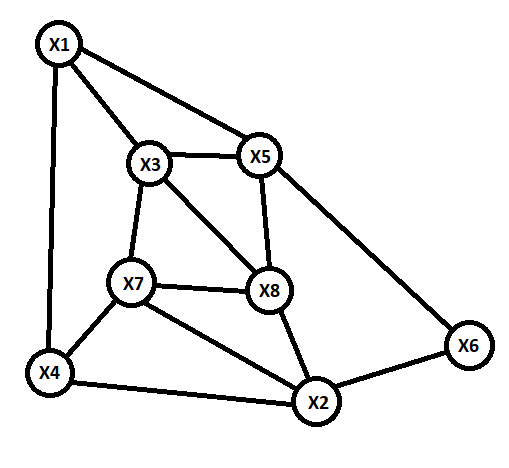
\includegraphics[width=10cm]{GRAF1.png}
\end{figure}

\newpage

    \textbf{Graf $G_2$: }
   
   \begin{figure}[htp]
    \centering
    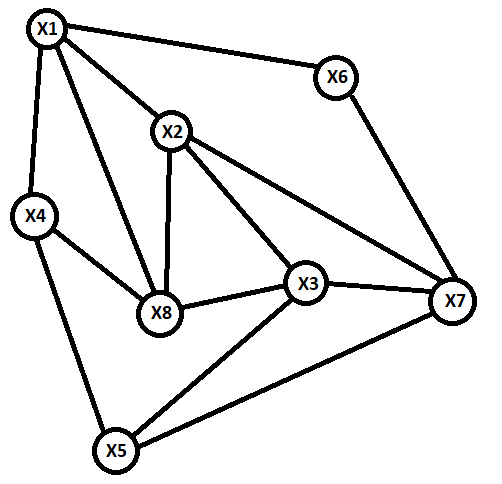
\includegraphics[width=10cm]{GRAF2.png}
\end{figure}

    \textbf{Graf $G_3$: }
    
   \begin{figure}[htp]
    \centering
    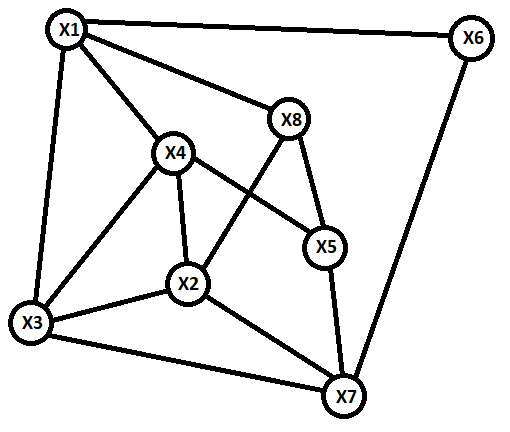
\includegraphics[width=9.2cm]{GRAF3.png}
\end{figure}

\vspace{0.5cm}
\textit{\\Prvi i drugi graf sadrže po 5 kontura dužine 3, dok graf 3 sadrži samo 3 takve konture pa samim time ne može biti izomorfan ni sa jednim od preostala dva grafa.\\Ostaje još da provjerimo da li se čvorovi u grafovima 1 i 2 mogu preimenovati tako da se dobije onaj drugi graf.}\\
\vspace{0.5cm}
    \textit{\\To je zaista i moguće, preimenovanjem čvorova $G_1$ na način:\\ \textbf{f:} $x_2 \rightarrow x_1; x_6 \rightarrow x_6; x_4 \rightarrow x_4; x_8 \rightarrow x_2; x_7 \rightarrow x_8, x_3 \rightarrow x_3; x_1 \rightarrow x_5; x_5 \rightarrow x_7$\\zaista dobijemo graf ekvivalentan grafu $G_2$, pa su $G_1$ i $G_2$ međusobno izomorfni grafovi.\\
    \vspace{0.5cm}
    c) Već smo pokazali da su grafovi $G_1$ i $G_2$ planarni sa skice, potrebno je još dokazati da je graf $G_3$ neplanaran graf. Vrijedi potreban uslov planarnosti jer je 14 $\leq (3 \cdot 8 - 6)$, odnosno $14 \leq 18$. Međutim, možemo pokazati da je $G_3$ svodiv na $K_5$. Ukoliko utopimo čvorove $x_2 \rightarrow x_8$, $x_5 \rightarrow x_7$ i $x_6 \rightarrow x_1$ po Wagnerovoj teoremi, zaista dobijamo K-5 graf i graf $G_3$ sigurno nije planaran.
    }
    
    \begin{figure}[htp]
    \centering
    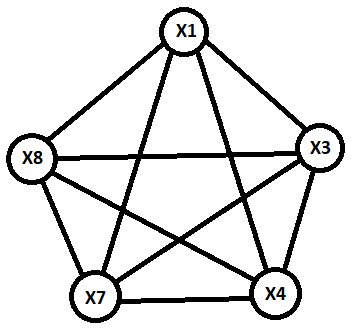
\includegraphics[width=8cm]{k5graf.png}
\end{figure}
    \\
    \textit{Illuminati confirmed}\\
    
    \vspace{0.3cm}
\textit{\\d) Obojimo grafove $G_1$ (odnosno i ekvivalentni $G_2$) pohlepnim algoritmom:}  \\

\begin{figure}[htp]
    \centering
    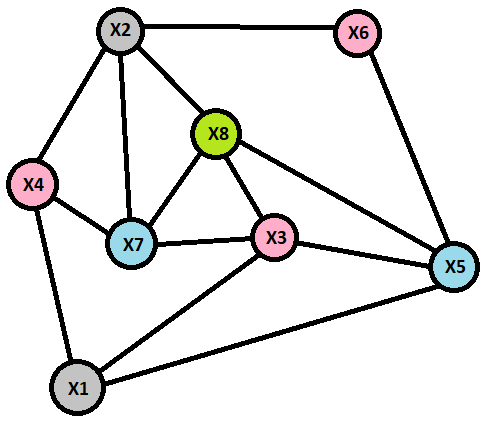
\includegraphics[width=10cm]{g1obojenekvivalentanG2.png}
\end{figure}

\textit{\\Najprije bojimo čvor $x_1$ u polaznu sivu boju, nakon toga kako $x_2$ nema obojenog nijednog susjeda onda njega možemo također obojiti u početnu sivu boju, slijedi čvor $x_3$ koji ima jednog sivog susjeda pa njega bojimo sljedećom bojom po redu a to je crvena, prelazimo na čvor $x_4$ za kojeg vrijedi isto kao za $x_3$ kako ima sivog susjeda bojimo ga u crvenu. Sljedeći čvor je čvor $x_5$ koji sada ima i sivog i crvenog susjeda pa ga bojimo u sljedeću boju a to je plava, nakon njega na redu je čvor $x_6$ koji ima plavog i sivog susjeda pa ga možemo obojiti u crvenu te na kraju ne manje bitan čvor $x_8$ ima i sivog i plavog i crvenog susjeda pa ga moramo obojiti u boju koju do sada nismo vidjeli odnosno Nihadu Alibegoviću dragu, zelenu.\\ Očigledno je hromatski broj grafova $G_1$ i $G_2$ jednak 4, imajući u vidu da tako mora biti (manji ili jednak 4) jer su grafovi planarni.}\\
\vspace{0.5cm}
\textit{Graf $G_3$}
    \begin{figure}[htp]
    \centering
    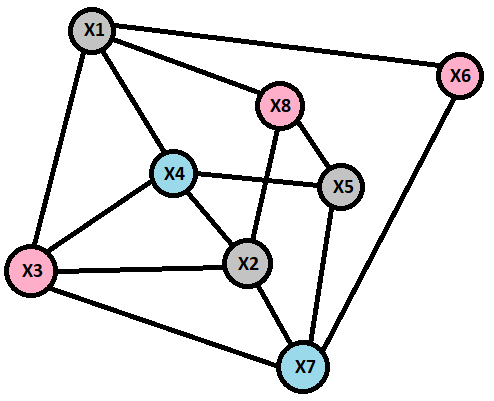
\includegraphics[width=10cm]{g3obojen.png}
\end{figure}
   
\vspace{0.5cm}
\textit{\\Prvo bojimo $x_1$ u početnu sivu boju i nakon toga prelazimo na $x_2$ koji nema obojenog nijednog susjeda pa i njega možemo obojiti u sivu boju, slijedi čvor $x_3$ koji ima sivog susjeda pa ga bojimu u sljedeću po redu boju a to je crvena. Na redu je $x_4$ koji ima i sivog i crvenog susjeda pa ga bojimo u plavu boju. Dolazi $x_5$ koji nema obojenog niti jednog susjeda pa ga možemo obojiti u početnu sivu boju. Sljedeći je $x_6$ koji ima sivog susjeda pa ga bojimo u crvenu boju, nakon čega čvor $x_7$ bojimo u plavu boju jer ima i sivog i crvenog susjeda. Te na kraju čvor $x_8$ bojimo u crvenu boju jer ima sive susjede.\\ Očito je hromatski broj grafa 3.}    
\end{center}
\vspace{0.75cm}
	\item Potrebno je povezati 12 lokacija L1 – L12 u računarsku mrežu. Zbog tehnoloških ograničenja, kablove nije moguće razvesti između proizvoljne dvije lokacije. Sljedeći spisak opisuje sve moguće načine kablovskog povezivanja lokacija, pri čemu trojka oblika (Li, Lj, dij) označava da je moguće spojiti lokacije Li i Lj, i to kablom dužine dij (u metrima): \\

(L1, L4, 670)   (L1, L9, 1290)   (L1, L12, 1030)   (L2, L5, 1210)   (L2, L6, 270)   (L2, L9, 660)   (L2, L10, 450)   (L2, L11, 750)   (L3, L4, 990)   (L3, L6, 790)   (L3, L7, 790)   (L3, L9, 1020)   (L4, L8, 570)   (L5, L6, 1170)   (L5, L8, 410)   (L5, L12, 850)   (L6, L7, 970)   (L6, L9, 870)   (L6, L10, 930)   (L7, L11, 300)   (L8, L9, 770)   (L8, L12, 1300)   (L9, L11, 1190)   (L9, L12, 450)   (L10, L11, 1100)   \\

Dizajnirajte računarsku mrežu u skladu sa navedenim specifikacijama tako da ukupan utrošak kablova bude minimalan i obavezno naznačite koliko iznosi taj utrošak. Dizajn obavite:\\
\ a)Primjenom Kruskalovog algoritma sa bojenjem čvorova;\\
\ b)Primjenom optimalnog Kruskalovog algoritma;\\
\ c)Primjenom optimiziranog (kvadratnog) Primovog algoritma.\\
U sva tri slučaja, nemojte crtati odgovarajući graf, nego sve neophodne radnje obavljajte “naslijepo”, koristeći samo raspoložive podatke, eventualno uz bilježenje izvjesnih pomoćnih informacija.

\begin{center}
    \textit{a) Najprije ćemo primijeniti Kruskalov algoritam sa bojenjem čvorova:\\}

\begin{tabular}{|c|c|c|c|c|c|c|c|c|c|c|c|c|c|c|}
\hline
Grana & Težina & Uzeti & c1 & c2 & c3 & c4 & c5 & c6 & c7 & c8 & c9 & c10 & c11 & c12 \\ \hline
\textbf{/} & \textbf{/} & \textbf{/} & 1 & 2 & 3 & 4 & 5 & 6 & 7 & 8 & 9 & 10 & 11 & 12 \\ \hline
2-6 & 270 & da &  & 1 &  &  &  & 1 &  &  &  &  &  &  \\ \hline
7-11 & 300 & da &  &  &  &  &  &  & 2 &  &  &  & 2 &  \\ \hline
5-8 & 410 & da &  &  &  &  & \textbf{3} &  &  & \textbf{3} &  &  &  &  \\ \hline
2-10 & 450 & da &  &  &  &  &  &  &  &  &  & 1 &  &  \\ \hline
9-12 & 450 & da &  &  &  &  &  &  &  &  & 4 &  &  & 4 \\ \hline
4-8 & 570 & da &  &  &  & \textbf{3} &  &  &  &  &  &  &  &  \\ \hline
2-9 & 660 & da &  &  &  &  &  &  &  &  & 1 &  &  & 1 \\ \hline
1-4 & 670 & da & \textbf{3} &  &  &  &  &  &  &  &  &  &  &  \\ \hline
2-11 & 750 & da &  &  &  &  &  &  & 1 &  &  &  & 1 &  \\ \hline
8-9 & 770 & da &  & \textbf{3} &  &  &  & \textbf{3} & \textbf{3} &  & \textbf{3} & \textbf{3} & \textbf{3} & \textbf{3} \\ \hline
3-7 & 790 & da &  &  & \textbf{3} &  &  &  &  &  &  &  &  &  \\ \hline
3-6 & 790 & ne &  &  &  &  &  &  &  &  &  &  &  &  \\ \hline
5-12 & 850 & ne &  &  &  &  &  &  &  &  &  &  &  &  \\ \hline
6-9 & 870 & ne &  &  &  &  &  &  &  &  &  &  &  &  \\ \hline
6-10 & 930 & ne &  &  &  &  &  &  &  &  &  &  &  &  \\ \hline
6-7 & 970 & ne &  &  &  &  &  &  &  &  &  &  &  &  \\ \hline
3-4 & 990 & ne &  &  &  &  &  &  &  &  &  &  &  &  \\ \hline
3-9 & 1020 & ne &  &  &  &  &  &  &  &  &  &  &  &  \\ \hline
1-12 & 1030 & ne &  &  &  &  &  &  &  &  &  &  &  &  \\ \hline
10-11 & 1100 & ne &  &  &  &  &  &  &  &  &  &  &  &  \\ \hline
5-6 & 1170 & ne &  &  &  &  &  &  &  &  &  &  &  &  \\ \hline
9-11 & 1190 & ne &  &  &  &  &  &  &  &  &  &  &  &  \\ \hline
2-5 & 1210 & ne &  &  &  &  &  &  &  &  &  &  &  &  \\ \hline
1-9 & 1290 & ne &  &  &  &  &  &  &  &  &  &  &  &  \\ \hline
8-12 & 1300 & ne &  &  &  &  &  &  &  &  &  &  &  &  \\ \hline
\end{tabular}


\vspace{0.5cm}
\textit{\\Optimalni način povezivanja je koristeći kablove (2,6), (7,11), (5,8), (2,10), (9,12), (4,8), (2,9), (1,4), (2,11), (8,9),  (3,7).\\Ukupan utrošak kablova iznosi:\\ 270 + 300 + 410 + 450 + 450 + 570 + 660 + 670 + 750 + 770 + 790 = \fbox{6090}}\\
\vspace{0.3cm}
\textit{b) Sada riješimo problem primjenom optimalnog Kruskalovog algoritma:\\}

\resizebox{.9\textwidth}{!}{%
\begin{tabular}{|c|c|c|c|c|c|c|c|c|c|c|c|c|c|c|}
\hline
Grana & Težina & Uzeti & c1/1 & c2/1 & c3/1 & c4/1 & c5/1 & c6/1 & c7/1 & c8/1 & c9/1 & c10/1 & c11/1 & c12/1 \\ \hline
\textbf{/} & \textbf{/} & \textbf{/} & 1 & 2 & 3 & 4 & 5 & 6 & 7 & 8 & 9 & 10 & 11 & 12 \\ \hline
2-6 & 270 & da &  & c2/2 &  &  &  & c2/1 &  &  &  &  &  &  \\ \hline
7-11 & 300 & da &  &  &  &  &  &  & c7/2 &  &  &  & c7/1 &  \\ \hline
5-8 & 410 & da &  &  &  &  & c5/2 &  &  & c5/1 &  &  &  &  \\ \hline
2-10 & 450 & da &  & c2/3 &  &  &  &  &  &  &  & c2/1 &  &  \\ \hline
9-12 & 450 & da &  &  &  &  &  &  &  &  & c9/2 &  &  & c9/1 \\ \hline
4-8 & 570 & da &  &  &  & c5/1 & c5/3 &  &  &  &  &  &  &  \\ \hline
2-9 & 660 & da &  & c2/5 &  &  &  &  &  &  & c2/2 &  &  &  \\ \hline
1-4 & 670 & da & c5/1 &  &  &  & c5/4 &  &  &  &  &  &  &  \\ \hline
2-11 & 750 & da &  & c2/7 &  &  &  &  & c2/2 &  &  &  &  &  \\ \hline
8-9 & 770 & da &  & c2/11 &  &  & c2/4 & \textbf{} & \textbf{} &  & \textbf{} & \textbf{} & \textbf{} & \textbf{} \\ \hline
3-7 & 790 & da &  & c2/12 & c2/1 &  &  &  &  &  &  &  &  &  \\ \hline
3-6 & 790 & ne &  &  &  &  &  &  &  &  &  &  &  &  \\ \hline
5-12 & 850 & ne &  &  &  &  &  &  &  &  &  &  &  &  \\ \hline
6-9 & 870 & ne &  &  &  &  &  &  &  &  &  &  &  &  \\ \hline
6-10 & 930 & ne &  &  &  &  &  &  &  &  &  &  &  &  \\ \hline
6-7 & 970 & ne &  &  &  &  &  &  &  &  &  &  &  &  \\ \hline
3-4 & 990 & ne &  &  &  &  &  &  &  &  &  &  &  &  \\ \hline
3-9 & 1020 & ne &  &  &  &  &  &  &  &  &  &  &  &  \\ \hline
1-12 & 1030 & ne &  &  &  &  &  &  &  &  &  &  &  &  \\ \hline
10-11 & 1100 & ne &  &  &  &  &  &  &  &  &  &  &  &  \\ \hline
5-6 & 1170 & ne &  &  &  &  &  &  &  &  &  &  &  &  \\ \hline
9-11 & 1190 & ne &  &  &  &  &  &  &  &  &  &  &  &  \\ \hline
2-5 & 1210 & ne &  &  &  &  &  &  &  &  &  &  &  &  \\ \hline
1-9 & 1290 & ne &  &  &  &  &  &  &  &  &  &  &  &  \\ \hline
8-12 & 1300 & ne &  &  &  &  &  &  &  &  &  &  &  &  \\ \hline

\end{tabular}%
}\\
\vspace{0.5cm}
\textit{Utrošak kablova u ovom slučaju je jednak slučaju pod a) jer se koristi isti put obilaska.}\\
\vspace{0.5cm}
\textit{c) Naposlijetku, riješimo zadatak primjenom kvadratnog Primovog algoritma. Na početku uzimamo $x_1$ kao referentni čvor:}\\


\resizebox{.9\textwidth}{!}{%
\begin{tabular}{|c|c|c|c|ccccccccc}
\hline
\multirow{2}{*}{Ref. čvor} & c1 & c2 & c3 & \multicolumn{1}{c|}{c4} & \multicolumn{1}{c|}{c5} & \multicolumn{1}{c|}{c6} & \multicolumn{1}{c|}{c7} & \multicolumn{1}{c|}{c8} & \multicolumn{1}{c|}{c9} & \multicolumn{1}{c|}{c10} & \multicolumn{1}{c|}{c11} & \multicolumn{1}{c|}{c12} \\ \cline{2-13} 
 & \textbf{0} &  &  & \multicolumn{1}{c|}{} & \multicolumn{1}{c|}{} & \multicolumn{1}{c|}{} & \multicolumn{1}{c|}{} & \multicolumn{1}{c|}{} & \multicolumn{1}{c|}{} & \multicolumn{1}{c|}{} & \multicolumn{1}{c|}{} & \multicolumn{1}{c|}{} \\ \hline
x1 &  &  &  & \multicolumn{1}{c|}{\textbf{670/x1}} & \multicolumn{1}{c|}{} & \multicolumn{1}{c|}{} & \multicolumn{1}{c|}{} & \multicolumn{1}{c|}{} & \multicolumn{1}{c|}{1290/x1} & \multicolumn{1}{c|}{} & \multicolumn{1}{c|}{} & \multicolumn{1}{c|}{1030/x1} \\ \hline
x4 &  &  & 990/x4 & \multicolumn{1}{c|}{} & \multicolumn{1}{c|}{} & \multicolumn{1}{c|}{} & \multicolumn{1}{c|}{} & \multicolumn{1}{c|}{\textbf{570/x4}} & \multicolumn{1}{c|}{1290/x1} & \multicolumn{1}{c|}{} & \multicolumn{1}{c|}{} & \multicolumn{1}{c|}{1030/x1} \\ \cline{1-4} \cline{6-13} 
x8 &  &  & 990/x4 & \multicolumn{1}{c|}{} & \multicolumn{1}{c|}{\textbf{410/x8}} & \multicolumn{1}{c|}{} & \multicolumn{1}{c|}{} & \multicolumn{1}{c|}{} & \multicolumn{1}{c|}{770/x8} & \multicolumn{1}{c|}{} & \multicolumn{1}{c|}{} & \multicolumn{1}{c|}{1030/x1} \\ \cline{1-4} \cline{6-8} \cline{10-13} 
x5 &  & 1210/x5 & 990/x4 &  & \multicolumn{1}{c|}{} & \multicolumn{1}{c|}{1170/x5} & \multicolumn{1}{c|}{} & \multicolumn{1}{c|}{} & \multicolumn{1}{c|}{\textbf{770/x8}} & \multicolumn{1}{c|}{} & \multicolumn{1}{c|}{} & \multicolumn{1}{c|}{850/x5} \\ \cline{1-4} \cline{7-8} \cline{10-13} 
x9 &  & 660/x9 & 1020/x9 &  & \multicolumn{1}{c|}{} & \multicolumn{1}{c|}{870/x9} & \multicolumn{1}{c|}{} &  & \multicolumn{1}{c|}{\textbf{}} & \multicolumn{1}{c|}{} & \multicolumn{1}{c|}{1190/x9} & \multicolumn{1}{c|}{\textbf{450/x9}} \\ \cline{1-4} \cline{7-8} \cline{11-13} 
x12 &  & \textbf{660/x9} & 1020/x9 &  & \multicolumn{1}{c|}{} & \multicolumn{1}{c|}{870/x9} & \multicolumn{1}{c|}{} &  & \multicolumn{1}{c|}{} & \multicolumn{1}{c|}{} & \multicolumn{1}{c|}{1190/x9} &  \\ \cline{1-4} \cline{7-8} \cline{11-12}
x2 &  &  & 1020/x9 &  & \multicolumn{1}{c|}{} & \multicolumn{1}{c|}{\textbf{270/x2}} & \multicolumn{1}{c|}{} &  & \multicolumn{1}{c|}{} & \multicolumn{1}{c|}{450/x2} & \multicolumn{1}{c|}{750/x2} &  \\ \cline{1-2} \cline{4-4} \cline{7-8} \cline{11-12}
x6 &  & \textbf{} & 790/x6 &  &  & \multicolumn{1}{c|}{} & \multicolumn{1}{c|}{970/x6} &  & \multicolumn{1}{c|}{} & \multicolumn{1}{c|}{\textbf{450/x2}} & \multicolumn{1}{c|}{750/x2} &  \\ \cline{1-2} \cline{4-4} \cline{8-8} \cline{11-12}
x10 &  &  & 790/x6 &  &  & \multicolumn{1}{c|}{} & \multicolumn{1}{c|}{970/x6} &  &  & \multicolumn{1}{c|}{} & \multicolumn{1}{c|}{\textbf{750/x2}} &  \\ \cline{1-2} \cline{4-4} \cline{8-8} \cline{12-12}
x11 &  &  & 790/x6 &  &  & \multicolumn{1}{c|}{} & \multicolumn{1}{c|}{\textbf{300/x11}} &  &  &  & \textbf{} &  \\ \cline{1-2} \cline{4-4} \cline{8-8}
x7 &  &  & \textbf{790/x6} &  &  &  &  &  & \textbf{} & \textbf{} &  &  \\ \cline{1-2} \cline{4-4}

\end{tabular}%
}\\
\vspace{0.5cm}
\textit{Dobijamo isto minimalno povezujuće stablo kao i kod Kruskalovog algoritma. Međutim to ne mora biti slučaj jer MPS ne mora biti jedinstveno kada su težine barem dvije grane jednake. Zbog redoslijeda uzimanja smo dobili jednako stablo. Ne bismo napravili grešku ni da smo te dvije grane uzeli suprotnim redoslijedom obzirom da je suma težina i dalje ista kao u a) i b).}

\end{center}
\newpage
\vspace{0.75cm}
	\item Turistička agencija “Pljačkaš tours” ima poslovnice u 8 gradova: Zavkul, Quwuti, Amcazo, Sosyab, Uyradu, Joxocap, Topufun i Rekazga. U sljedećoj tablici su date cijene direktnih avionskih letova između pojedinih gradova izražene u škafiškafnjacima (crtica znači da direktan let ne postoji):\\
	\vspace{0.3cm}\\
\begin{tabular}{|c|c|c|c|c|c|c|c|c|}
\hline
 & Zavkul & Quwuti & Amcazo & Sosyab & Uyradu & Joxocap & Topufun & Rekazga \\ \hline
Zavkul & 0 & - & 470 & 370 & 340 & 1270 & 360 & 430 \\ \hline
Quwuti & - & 0 & 370 & 300 & 700 & 430 & - & 260 \\ \hline
Amcazo & 470 & 370 & 0 & 400 & 960 & - & 1100 & 230 \\ \hline
Sosyab & 370 & 300 & 400 & 0 & - & 1120 & 420 & 440 \\ \hline
Uyradu & 340 & 700 & 960 & - & 0 & 230 & 230 & 680 \\ \hline
Joxocap & 1270 & 430 & - & 1120 & 230 & 0 & 690 & 340 \\ \hline
Topufun & 360 & - & 1100 & 420 & 230 & 690 & 0 & 300 \\ \hline
Rekazga & 430 & 260 & 230 & 440 & 680 & 340 & 300 & 0 \\ \hline
\end{tabular}
\\
     \vspace{0.3cm}\\
     Međutim, poznato je da direktni letovi nisu uvijek i najjeftiniji način aviotransporta između gradova, nego je nekada povoljnije koristiti presjedanje (pogotovo ako se na taj način mogu koristiti usluge low-cost kompanija. Na primjer, iz Topufuna jeftinije je u Joxocap putovati sa presjedanjem u Uyraduu nego direktnim letom (sa presjedanjem plaćamo 230 + 230 = 460 škafiškafnjaka, dok direktan let košta 690 škafiškafnjaka). Zbog toga, turistička agencija želi da sastavi tablicu koja sadrži informacije koliko iznose najjeftinije cijene aviotransporta između svakog para gradova u kojima agencija ima poslovnice (uz dopuštanje presjedanja) kao i u kojim gradovima treba eventualno vršiti presjedanja za svaki od tih transporta. Pomozite agenciji “Pljačkaš tours” da sastavi ove tablice. Postupak obavite uz pomoć Dijkstrinog algoritma, ali bez crtanja grafova, nego samo vršeći manipulacije nad zadanom tablicom, uz eventualno bilježenje pomoćnih dopunskih informacija.
     \vspace{0.75cm}
     \begin{center}
         \textit{Prije primjene Dijkstrinog algoritma označimo gradove pogodnim slovima:\\
         A-Zavkul,\
         B-Quwuti,\
         C-Amcazo,\
         D-Sosyab,\
         E-Uyradu,\
         F-Joxocap,\
         G-Topofun,\
         H-Rekazga\\}
         \vspace{0.5cm}
         A-Zavkul
         
\begin{tabular}{|l|l|l|llllll}
\hline
 & A & B & \multicolumn{1}{l|}{C} & \multicolumn{1}{l|}{D} & \multicolumn{1}{l|}{E} & \multicolumn{1}{l|}{F} & \multicolumn{1}{l|}{G} & \multicolumn{1}{l|}{H} \\ \hline
A(0) & 0 & - & \multicolumn{1}{l|}{470/A} & \multicolumn{1}{l|}{370/A} & \multicolumn{1}{l|}{\textbf{340/A}} & \multicolumn{1}{l|}{1270/A} & \multicolumn{1}{l|}{360/A} & \multicolumn{1}{l|}{430/A} \\ \hline
E(340) &  & 1040/E & \multicolumn{1}{l|}{470/A} & \multicolumn{1}{l|}{370/A} & \multicolumn{1}{l|}{} & \multicolumn{1}{l|}{570/E} & \multicolumn{1}{l|}{\textbf{360/A}} & \multicolumn{1}{l|}{430/A} \\ \cline{1-1} \cline{3-5} \cline{7-9} 
G(360) &  & 1040/E & \multicolumn{1}{l|}{470/A} & \multicolumn{1}{l|}{\textbf{370/A}} & \multicolumn{1}{l|}{} & \multicolumn{1}{l|}{570/E} & \multicolumn{1}{l|}{} & \multicolumn{1}{l|}{430/A} \\ \cline{1-1} \cline{3-5} \cline{7-7} \cline{9-9} 
D(370) &  & 670/D & \multicolumn{1}{l|}{470/A} &  & \multicolumn{1}{l|}{} & \multicolumn{1}{l|}{570/E} & \multicolumn{1}{l|}{} & \multicolumn{1}{l|}{\textbf{430/A}} \\ \cline{1-1} \cline{3-4} \cline{7-7} \cline{9-9} 
H(430) &  & 670/D & \multicolumn{1}{l|}{\textbf{470/A}} &  & \multicolumn{1}{l|}{} & \multicolumn{1}{l|}{570/E} &  &  \\ \cline{1-1} \cline{3-4} \cline{7-7}
C(470) &  & 670/D &  &  & \multicolumn{1}{l|}{} & \multicolumn{1}{l|}{\textbf{570/E}} &  &  \\ \cline{1-1} \cline{3-3} \cline{7-7}
F(570) &  & \textbf{670/D} &  &  &  & \textbf{} &  &  \\ \cline{1-1} \cline{3-3}
\end{tabular}
\\
      \vspace{0.5cm}   
         \newpage
         
            B-Quwuti
            
\begin{tabular}{|l|l|lllllll}
\hline
 & A & \multicolumn{1}{l|}{B} & \multicolumn{1}{l|}{C} & \multicolumn{1}{l|}{D} & \multicolumn{1}{l|}{E} & \multicolumn{1}{l|}{F} & \multicolumn{1}{l|}{G} & \multicolumn{1}{l|}{H} \\ \hline
B(0) & - & \multicolumn{1}{l|}{0} & \multicolumn{1}{l|}{370/B} & \multicolumn{1}{l|}{300/B} & \multicolumn{1}{l|}{700/B} & \multicolumn{1}{l|}{430/B} & \multicolumn{1}{l|}{-} & \multicolumn{1}{l|}{\textbf{260/B}} \\ \hline
H(260) & 690/H & \multicolumn{1}{l|}{} & \multicolumn{1}{l|}{370/B} & \multicolumn{1}{l|}{\textbf{300/B}} & \multicolumn{1}{l|}{700/B} & \multicolumn{1}{l|}{430/B} & \multicolumn{1}{l|}{560/H} &  \\ \cline{1-2} \cline{4-8}
D(300) & 670/D & \multicolumn{1}{l|}{} & \multicolumn{1}{l|}{\textbf{370/B}} & \multicolumn{1}{l|}{} & \multicolumn{1}{l|}{700/B} & \multicolumn{1}{l|}{430/B} & \multicolumn{1}{l|}{560/H} &  \\ \cline{1-2} \cline{4-4} \cline{6-8}
C(370) & 670/D &  &  & \multicolumn{1}{l|}{} & \multicolumn{1}{l|}{700/B} & \multicolumn{1}{l|}{\textbf{430/B}} & \multicolumn{1}{l|}{560/H} &  \\ \cline{1-2} \cline{6-8}
F(430) & 670/D &  &  & \multicolumn{1}{l|}{} & \multicolumn{1}{l|}{660/F} & \multicolumn{1}{l|}{} & \multicolumn{1}{l|}{\textbf{560/H}} &  \\ \cline{1-2} \cline{6-6} \cline{8-8}
G(560) & 670/D &  &  & \multicolumn{1}{l|}{} & \multicolumn{1}{l|}{\textbf{660/F}} &  &  &  \\ \cline{1-2} \cline{6-6}
E(660) & \textbf{670/D} &  &  &  &  & \textbf{} &  &  \\ \cline{1-2}
\end{tabular}
\\
      \vspace{0.5cm}
      
              C-Amcazo
              
\begin{tabular}{|l|llll|l|lll}
\hline
 & \multicolumn{1}{l|}{A} & \multicolumn{1}{l|}{B} & \multicolumn{1}{l|}{C} & D & E & \multicolumn{1}{l|}{F} & \multicolumn{1}{l|}{G} & \multicolumn{1}{l|}{H} \\ \hline
C(0) & \multicolumn{1}{l|}{470/C} & \multicolumn{1}{l|}{370/C} & \multicolumn{1}{l|}{0} & 400/C & 960/C & \multicolumn{1}{l|}{-} & \multicolumn{1}{l|}{1100/C} & \multicolumn{1}{l|}{\textbf{230/C}} \\ \hline
H(230) & \multicolumn{1}{l|}{470/C} & \multicolumn{1}{l|}{\textbf{370/C}} & \multicolumn{1}{l|}{} & 400/C & 910/H & \multicolumn{1}{l|}{570/H} & \multicolumn{1}{l|}{530/H} &  \\ \cline{1-3} \cline{5-8}
B(370) & \multicolumn{1}{l|}{470/C} &  & \multicolumn{1}{l|}{} & \textbf{400/C} & 910/H & \multicolumn{1}{l|}{570/H} & \multicolumn{1}{l|}{530/H} &  \\ \cline{1-2} \cline{5-8}
D(400) & \multicolumn{1}{l|}{\textbf{470/C}} &  &  &  & 910/H & \multicolumn{1}{l|}{570/H} & \multicolumn{1}{l|}{530/H} &  \\ \cline{1-2} \cline{6-8}
A(470) &  &  &  &  & 810/A & \multicolumn{1}{l|}{570/H} & \multicolumn{1}{l|}{\textbf{530/H}} &  \\ \cline{1-1} \cline{6-8}
G(530) &  &  &  &  & 760/G & \multicolumn{1}{l|}{\textbf{570/H}} &  &  \\ \cline{1-1} \cline{6-7}
F(570) & \textbf{} &  &  &  & \textbf{760/G} & \textbf{} &  &  \\ \cline{1-1} \cline{6-6}
\end{tabular}
\\
      \vspace{0.5cm}
      
            D-Sosyab

\begin{tabular}{|l|llll|l|lll}
\hline
 & \multicolumn{1}{l|}{A} & \multicolumn{1}{l|}{B} & \multicolumn{1}{l|}{C} & D & E & \multicolumn{1}{l|}{F} & \multicolumn{1}{l|}{G} & \multicolumn{1}{l|}{H} \\ \hline
D(0) & \multicolumn{1}{l|}{370/D} & \multicolumn{1}{l|}{\textbf{300/D}} & \multicolumn{1}{l|}{400/D} & 0 & - & \multicolumn{1}{l|}{1120/D} & \multicolumn{1}{l|}{420/D} & \multicolumn{1}{l|}{440/D} \\ \hline
B(300) & \multicolumn{1}{l|}{\textbf{370/D}} & \multicolumn{1}{l|}{\textbf{}} & \multicolumn{1}{l|}{400/D} &  & 1000/B & \multicolumn{1}{l|}{730/B} & \multicolumn{1}{l|}{420/D} & \multicolumn{1}{l|}{440/D} \\ \cline{1-2} \cline{4-4} \cline{6-9} 
A(370) &  & \multicolumn{1}{l|}{} & \multicolumn{1}{l|}{\textbf{400/D}} & \textbf{} & 710/A & \multicolumn{1}{l|}{730/B} & \multicolumn{1}{l|}{420/D} & \multicolumn{1}{l|}{440/D} \\ \cline{1-1} \cline{4-4} \cline{6-9} 
C(400) & \textbf{} &  &  &  & 710/A & \multicolumn{1}{l|}{730/B} & \multicolumn{1}{l|}{\textbf{420/D}} & \multicolumn{1}{l|}{440/D} \\ \cline{1-1} \cline{6-9} 
G(420) &  &  &  &  & 650/G & \multicolumn{1}{l|}{730/B} & \multicolumn{1}{l|}{\textbf{}} & \multicolumn{1}{l|}{\textbf{440/D}} \\ \cline{1-1} \cline{6-7} \cline{9-9} 
H(440) &  &  &  &  & 650/G & \multicolumn{1}{l|}{\textbf{730/B}} &  &  \\ \cline{1-1} \cline{6-7}
F(730) & \textbf{} &  &  &  & \textbf{650/G} & \textbf{} &  &  \\ \cline{1-1} \cline{6-6}
\end{tabular}
\\
      \vspace{0.5cm}
      
          E-Uyradu
          
\begin{tabular}{|l|ll|l|lllll}
\hline
 & \multicolumn{1}{l|}{A} & B & C & \multicolumn{1}{l|}{D} & \multicolumn{1}{l|}{E} & \multicolumn{1}{l|}{F} & \multicolumn{1}{l|}{G} & \multicolumn{1}{l|}{H} \\ \hline
E(0) & \multicolumn{1}{l|}{340/E} & 700/E & 960/E & \multicolumn{1}{l|}{-} & \multicolumn{1}{l|}{0} & \multicolumn{1}{l|}{\textbf{230/E}} & \multicolumn{1}{l|}{230/E} & \multicolumn{1}{l|}{680/E} \\ \hline
F(230) & \multicolumn{1}{l|}{340/E} & 660/F & 960/E & \multicolumn{1}{l|}{1350/F} &  & \multicolumn{1}{l|}{} & \multicolumn{1}{l|}{\textbf{230/E}} & \multicolumn{1}{l|}{570/F} \\ \cline{1-5} \cline{8-9} 
G(230) & \multicolumn{1}{l|}{\textbf{340/E}} & 660/E & 960/E & \multicolumn{1}{l|}{650/G} &  &  & \multicolumn{1}{l|}{} & \multicolumn{1}{l|}{530/G} \\ \cline{1-5} \cline{9-9} 
A(340) & \multicolumn{1}{l|}{\textbf{}} & 660/E & 810/A & \multicolumn{1}{l|}{650/G} &  &  & \multicolumn{1}{l|}{} & \multicolumn{1}{l|}{\textbf{530/G}} \\ \cline{1-1} \cline{3-5} \cline{9-9} 
H(530) & \multicolumn{1}{l|}{} & 660/E & 760/H & \multicolumn{1}{l|}{\textbf{650/G}} &  &  & \textbf{} &  \\ \cline{1-1} \cline{3-5}
D(650) & \multicolumn{1}{l|}{} & \textbf{660/E} & 760/H &  &  &  &  &  \\ \cline{1-1} \cline{3-4}
B(660) & \textbf{} &  & \textbf{760/H} &  &  & \textbf{} &  &  \\ \cline{1-1} \cline{4-4}
\end{tabular}
\\
      \vspace{0.5cm}
      \newpage
      
       F-Joxocap
       
\begin{tabular}{|l|lll|l|llll}
\hline
 & \multicolumn{1}{l|}{A} & \multicolumn{1}{l|}{B} & C & D & \multicolumn{1}{l|}{E} & \multicolumn{1}{l|}{F} & \multicolumn{1}{l|}{G} & \multicolumn{1}{l|}{H} \\ \hline
F(0) & \multicolumn{1}{l|}{1270/F} & \multicolumn{1}{l|}{430/F} & - & 1120/F & \multicolumn{1}{l|}{\textbf{230/F}} & \multicolumn{1}{l|}{0} & \multicolumn{1}{l|}{690/F} & \multicolumn{1}{l|}{340/F} \\ \hline
E(230) & \multicolumn{1}{l|}{570/E} & \multicolumn{1}{l|}{430/F} & 1190/E & 1120/F &  & \multicolumn{1}{l|}{} & \multicolumn{1}{l|}{460/E} & \multicolumn{1}{l|}{\textbf{340/F}} \\ \cline{1-5} \cline{8-9} 
H(340) & \multicolumn{1}{l|}{570/E} & \multicolumn{1}{l|}{\textbf{430/F}} & 570/H & 780/H &  & \multicolumn{1}{l|}{} & \multicolumn{1}{l|}{460/E} &  \\ \cline{1-5} \cline{8-8}
B(430) & \multicolumn{1}{l|}{570/E} & \multicolumn{1}{l|}{} & 570/H & 730/B &  & \multicolumn{1}{l|}{} & \multicolumn{1}{l|}{\textbf{460/E}} &  \\ \cline{1-2} \cline{4-5} \cline{8-8}
G(460) & \multicolumn{1}{l|}{\textbf{570/E}} & \multicolumn{1}{l|}{} & 570/H & 730/B &  &  & \textbf{} &  \\ \cline{1-2} \cline{4-5}
A(570) &  & \multicolumn{1}{l|}{} & \textbf{570/H} & 730/B &  &  &  &  \\ \cline{1-1} \cline{4-5}
C(570) & \textbf{} &  &  & \textbf{730/B} &  & \textbf{} &  &  \\ \cline{1-1} \cline{5-5}
\end{tabular}
\\
 
         G-Topofun
         
\begin{tabular}{|l|l|l|llllll}
\hline
 & A & B & \multicolumn{1}{l|}{C} & \multicolumn{1}{l|}{D} & \multicolumn{1}{l|}{E} & \multicolumn{1}{l|}{F} & \multicolumn{1}{l|}{G} & \multicolumn{1}{l|}{H} \\ \hline
G(0) & 360/G & - & \multicolumn{1}{l|}{1100/G} & \multicolumn{1}{l|}{420/G} & \multicolumn{1}{l|}{\textbf{230/G}} & \multicolumn{1}{l|}{690/G} & \multicolumn{1}{l|}{0} & \multicolumn{1}{l|}{300/G} \\ \hline
E(230) & 360/G & 930/E & \multicolumn{1}{l|}{1100/G} & \multicolumn{1}{l|}{420/G} & \multicolumn{1}{l|}{} & \multicolumn{1}{l|}{460/E} & \multicolumn{1}{l|}{} & \multicolumn{1}{l|}{\textbf{300/G}} \\ \cline{1-5} \cline{7-7} \cline{9-9} 
H(300) & \textbf{360/G} & 560/H & \multicolumn{1}{l|}{530/H} & \multicolumn{1}{l|}{420/G} & \multicolumn{1}{l|}{} & \multicolumn{1}{l|}{460/E} &  &  \\ \cline{1-5} \cline{7-7}
A(360) &  & 560/H & \multicolumn{1}{l|}{530/H} & \multicolumn{1}{l|}{\textbf{420/G}} & \multicolumn{1}{l|}{} & \multicolumn{1}{l|}{460/E} &  &  \\ \cline{1-1} \cline{3-5} \cline{7-7}
D(420) &  & 560/H & \multicolumn{1}{l|}{530/H} &  & \multicolumn{1}{l|}{} & \multicolumn{1}{l|}{\textbf{460/E}} & \textbf{} &  \\ \cline{1-1} \cline{3-4} \cline{7-7}
F(460) &  & 560/H & \multicolumn{1}{l|}{\textbf{530/H}} &  &  &  &  &  \\ \cline{1-1} \cline{3-4}
C(530) & \textbf{} & \textbf{560/H} &  &  &  & \textbf{} &  &  \\ \cline{1-1} \cline{3-3}
\end{tabular}
\\
      \vspace{0.5cm}
      
             H-Rekazga
             
\begin{tabular}{|l|llll|l|lll}
\hline
 & \multicolumn{1}{l|}{A} & \multicolumn{1}{l|}{B} & \multicolumn{1}{l|}{C} & D & E & \multicolumn{1}{l|}{F} & \multicolumn{1}{l|}{G} & \multicolumn{1}{l|}{H} \\ \hline
H(0) & \multicolumn{1}{l|}{430/H} & \multicolumn{1}{l|}{260/H} & \multicolumn{1}{l|}{\textbf{230/H}} & 440/H & 680/H & \multicolumn{1}{l|}{340/H} & \multicolumn{1}{l|}{300/H} & \multicolumn{1}{l|}{0} \\ \hline
C(230) & \multicolumn{1}{l|}{430/H} & \multicolumn{1}{l|}{\textbf{260/H}} & \multicolumn{1}{l|}{} & 440/H & 680/H & \multicolumn{1}{l|}{340/H} & \multicolumn{1}{l|}{300/H} & \textbf{} \\ \cline{1-3} \cline{5-8}
B(260) & \multicolumn{1}{l|}{430/H} &  & \multicolumn{1}{l|}{} & 440/H & 680/H & \multicolumn{1}{l|}{340/H} & \multicolumn{1}{l|}{\textbf{300/H}} &  \\ \cline{1-2} \cline{5-8}
G(300) & \multicolumn{1}{l|}{430/H} &  & \multicolumn{1}{l|}{} & 440/H & 530/G & \multicolumn{1}{l|}{\textbf{340/H}} &  &  \\ \cline{1-2} \cline{5-7}
F(340) & \multicolumn{1}{l|}{\textbf{430/H}} &  & \multicolumn{1}{l|}{} & 440/H & 530/G & \textbf{} & \textbf{} &  \\ \cline{1-2} \cline{5-6}
A(430) &  &  & \multicolumn{1}{l|}{\textbf{}} & \textbf{440/G} & 530/G &  &  &  \\ \cline{1-1} \cline{5-6}
D(440) & \textbf{} & \textbf{} &  &  & \textbf{530/G} & \textbf{} &  &  \\ \cline{1-1} \cline{6-6}
\end{tabular}
\\
      \vspace{1cm}
      \textit{Tablica najkraćih puteva između pojedinih gradova:\\}
\resizebox{1\textwidth}{!}{%
\begin{tabular}{|c|c|c|c|c|c|c|c|c|}
\hline
 & A-Zavkul & B-Quwuti & C-Amcazo & D-Sosyab & E-Uyradu & F-Joxocap & G-Topufun & H-Rekazga \\ \hline
A-Zavkul & 0 & 670/D & 470/A & 370/A & 340/A & 570/E & 360/A & 430/A \\ \hline
B-Quwuti & 670/D & 0 & 370/B & 300/B & 660/B & 430/B & 560/B & 260/B \\ \hline
C-Amcazo & 470/C & 370/C & 0 & 400/C & 760/G & 570/H & 530/H & 230/C \\ \hline
D-Sosyab & 370/D & 300/D & 400/D & 0 & 650/G & 730/B & 420/D & 440/D \\ \hline
E-Uyradu & 340/E & 660/E & 760/H & 650/G & 0 & 230/E & 230/E & 530/G \\ \hline
F-Joxocap & 570/E & 430/F & 570/H & 730/B & 230/F & 0 & 460/E & 340/F \\ \hline
G-Topufun & 360/G & 560/H & 530/H & 420/G & 230/G & 460/E & 0 & 300/G \\ \hline
H-Rekazga & 430/H & 260/H & 230/H & 440/G & 530/G & 340/H & 300/H & 0 \\ \hline
\end{tabular}%
      }\\
     \end{center}
     \newpage
	\item Dat je usmjereni težinski graf
G = \{\{A, B, C, D, E, F, G, H, I, J\}, \{(A, F, 64), (A, I, -52), (B, E, 16), (C, A, 44), (C, B, 60), (C, F, 52), (D, B, 52), (E, G, 48), (E, J, 36), (F, D, -84), (F, E, 48), (G, C, -24), (G, D, 32), (G, I, 40), (H, C, -68), (H, F, 20), (I, E, 56), (J, G, -76)\}\}
Koristeći Bellman-Fordov algoritam, dokažite da u ovom grafu postoji kontura sa negativnom sumom težina u konturi.\\ Nakon toga pronađite makar jednu takvu konturu. Postupak obavite “naslijepo”, bez crtanja grafa, koristeći samo raspoložive informacije (eventualno uz bilježenje raznih pomoćnih informacija).\\
\begin{center}
 \textit{Za dokazivanje da u grafu postoji barem jedna kontura sa negativnom sumom težina moramo dobiti da je $\lambda_A$ negativno u nekoj od iteracija algoritma:\\}
 \vspace{0.5cm}
\\


\begin{tabular}{|c|c|c|c|c|c|c|c|c|c|c|c|}
\hline
$x_j$ & A & B & C & D & E & F & G & H & I & J & \multirow{2}{*}{$\lambda_i$} \\ \cline{1-11}
$x_i$ & 0 & $\infty$ & $\infty$ & \textbf{$\infty$} & \textbf{$\infty$} & \textbf{$\infty$} &$\infty$ &$\infty$ & \textbf{$\infty$} & $\infty$ &  \\ \hline
A &  &  &  &  &  & 64 &  &  & -52 &  & $\infty$ \\ \hline
B &  &  &  &  & $\infty$ &  &  &  &  &  & $\infty$ \\ \hline
C & $\infty$ & $\infty$ &  &  &  & $\infty$ &  &  &  &  & $\infty$ \\ \hline
D &  & \textbf{$\infty$} &  &  &  &  &  &  &  &  & $\infty$,-20 \\ \hline
E &  &  &  &  &  &  & $\infty$ &  &  & $\infty$ & $\infty$,112,4 \\ \hline
F &  &  &  & -20 & 112 &  &  &  &  &  & $\infty$,64 \\ \hline
G &  &  & $\infty$ & $\infty$ &  &  &  &  & $\infty$ &  & $\infty$ \\ \hline
H &  &  & $\infty$ &  &  & $\infty$ &  &  &  &  & $\infty$ \\ \hline
I &  &  &  &  & 4 &  &  &  &  &  & $\infty$,-52 \\ \hline
J &  &  &  &  &  &  &$\infty$&  &  &  & $\infty$ \\ \hline
\end{tabular}\\
 \vspace{0.3cm}

\begin{tabular}{|c|c|c|c|c|c|c|c|c|c|c|c|}
\hline
$x_j$ & A & B & C & D & E & F & G & H & I & J & \multirow{2}{*}{$\lambda_i$} \\ \cline{1-11}
$x_i$ & 0 & $\infty$ & $\infty$& \textbf{-20} & \textbf{4} & \textbf{64} & $\infty$ & $\infty$ & \textbf{-52} & $\infty$ &  \\ \hline
A &  &  &  &  &  &  &  &  &  &  & $\infty$ \\ \hline
B &  &  &  &  &  &  &  &  &  &  & $\infty$,32 \\ \hline
C &  &  &  &  &  &  &  &  &  &  & $\infty$,28 \\ \hline
D &  & 32 &  &  &  &  &  &  &  &  & -20 \\ \hline
E &  &  &  &  &  &  & 52 &  &  & 40 & 4 \\ \hline
F &  &  &  & -20 & 112 &  &  &  &  &  & 64 \\ \hline
G &  &  & 28 & 84 &  &  &  &  & 92 &  & $\infty$,52,-36 \\ \hline
H &  &  &  &  &  &  &  &  &  &  & $\infty$ \\ \hline
I &  &  &  &  & 4 &  &  &  &  &  & -52 \\ \hline
J &  &  &  &  &  &  & -36 &  &  &  & $\infty$,40 \\ \hline
\end{tabular}\\
\vspace{0.3cm}

\begin{tabular}{|c|c|c|c|c|c|c|c|c|c|c|c|}
\hline
$x_j$ & A & B & C & D & E & F & G & H & I & J & \multirow{2}{*}{$\lambda_i$} \\ \cline{1-11}
$x_i$ & 0 & 32 & 28 & \textbf{-20} & \textbf{4} & \textbf{64} & \textbf{-36} & besk & \textbf{-52} & 40 &  \\ \hline
A &  &  &  &  &  &  &  &  &  &  &  \\ \hline
B &  &  &  &  & 48 &  &  &  &  &  & 32 \\ \hline
C & 72 & 88 &  &  &  & 80 &  &  &  &  & 28,-60 \\ \hline
D &  & \textbf{} &  &  &  &  &  &  &  &  &  \\ \hline
E &  &  &  &  &  &  &  &  &  & \textbf{} &  \\ \hline
F &  &  &  &  &  &  &  &  &  &  &  \\ \hline
G &  &  & \textbf{-60} & -4 &  &  &  &  & 4 &  & -36 \\ \hline
H &  &  &  &  &  &  &  &  &  &  &  \\ \hline
I &  &  &  &  &  &  &  &  &  &  &  \\ \hline
J &  &  &  &  &  &  & -36 &  &  &  & 40 \\ \hline
\end{tabular}\\
\vspace{0.3cm}
\begin{tabular}{|c|c|c|c|c|c|c|c|c|c|c|c|}
\hline
$x_j$ & A & B & C & D & E & F & G & H & I & J & \multirow{2}{*}{$\lambda_i$} \\ \cline{1-11}
$x_i$ & 0 & 32 & -60 & \textbf{-20} & \textbf{4} & \textbf{64} & \textbf{-36} & besk & \textbf{-52} & 40 &  \\ \hline
A &  &  &  &  &  &  &  &  &  &  &  \\ \hline
B &  &  &  &  &  &  &  &  &  &  &  \\ \hline
C & \textbf{-16} &  &  &  &  &  &  &  &  &  & -60 \\ \hline
D &  & \textbf{} &  &  &  &  &  &  &  &  &  \\ \hline
E &  &  &  &  &  &  &  &  &  & \textbf{} &  \\ \hline
F &  &  &  &  &  &  &  &  &  &  &  \\ \hline
G &  &  & \textbf{} &  &  &  &  &  &  &  &  \\ \hline
H &  &  &  &  &  &  &  &  &  &  &  \\ \hline
I &  &  &  &  &  &  &  &  &  &  &  \\ \hline
J &  &  &  &  &  &  &  &  &  &  &  \\ \hline
\end{tabular}
\\
\vspace{0.3cm}

      \textit{Pošto smo u četvrtoj iteraciji dobili da je $\lambda_A$ negativno, time je dokazano da postoji barem jedna kontura sa negativnom sumom težina. Jedna takva kontura je \textbf{A-I-E-J-G-C-A} čija je suma:\\ -52 + 56 + 36 - 76 - 24 + 44 = -16.}
      
\end{center}
	\item Dat je usmjereni težinski graf

G= \{\{x1, x2, x3, x4, x5, x6, x7, x8, x9, x10, x11\}, \{(x2, x4, 29), (x2, x8, 11), (x3, x7, 24), (x3, x10, 5), (x4, x5, 6), (x4, x6, 24), (x5, x1, 7), (x5, x6, 15), (x6, x1, 6), (x6, x11, 13), (x7, x2, 16), (x7, x4, 22), (x8, x6, 38), (x8, x11, 17), (x9, x3, 21), (x9, x7, 30), (x9, x10, 5), (x10, x2, 5), (x10, x8, 34), (x11, x1, 11)\}\}\\
-Pokažite da u ovom grafu ima tačno jedan izvor (čvor ulaznog stepena 0) i tačno jedan ponor (čvor izlaznog stepena 0), te da se radi o acikličkom grafu;\\
-Izvršite topološko sortiranje čvorova ovog grafa obavljajući DFS pretragu počev od izvora grafa;\\
-Primjenom Dijkstrinog algoritma, pronađite najkraći put od izvora do ponora grafa i navedite koliko iznosi dužina tog puta;\\
-Primjenom Bellman-Fordovog algoritma, pronađite najkraći put od izvora do ponora grafa i navedite koliko iznosi dužina tog puta;\\
-Primjenom Bellman-Fordovog algoritma, pronađite najduži put od izvora do ponora grafa i navedite koliko iznosi dužina tog puta.\\
Postupak provedite “naslijepo”, bez crtanja grafa, koristeći samo raspoložive informacije (eventualno uz bilježenje raznih pomoćnih informacija).\\
\begin{center}
    \textit{Za lakše dokazivanje napišimo graf u formi matrične tabele:\\}
    
     \resizebox{.9\textwidth}{!}{%
\begin{tabular}{|l|l|l|l|l|l|l|l|l|l|l|l|}
\hline
 & $x_1$ & $x_2$ & $x_3$ & $x_4$ & $x_5$ & $x_6$ & $x_7$ & $x_8$ & $x_9$ & $x_{10}$ & $x_{11}$ \\ \hline
$x_1$ &  &  &  &  &  &  &  &  &  &  &  \\ \hline
$x_2$&  &  &  & 29 &  &  &  & 11 &  &  &  \\ \hline
$x_3$ &  &  &  &  &  &  & 24 &  &  & 5 &  \\ \hline
$x_4$ &  &  &  &  & 6 & 24 &  &  &  &  &  \\ \hline
$x_5$ & 7 &  &  &  &  & 15 &  &  &  &  &  \\ \hline
$x_6$ & 6 &  &  &  &  &  &  &  &  &  & 13 \\ \hline
$x_7$ &  & 16 &  & 22 &  &  &  &  &  &  &  \\ \hline
$x_8$ &  &  &  &  &  & 38 &  &  &  &  & 17 \\ \hline
$x_9$ &  &  & 21 &  &  &  & 30 &  &  & 5 &  \\ \hline
$x_{10}$ &  & 5 &  &  &  &  &  & 34 &  &  &  \\ \hline
$x_{11}$ & 11 &  &  &  &  &  &  &  &  &  &  \\ \hline
\end{tabular}%
      }\\
      \vspace{0.5cm}
    \textit{Očigledno je (iz tabele) izvor čvor $x_9$, a ponor čvor $x_1$.}\\
    \vspace{0.3cm}
    \\

    \textit{Sada izvršimo topološko sortiranje čvorova putem DFS pretrage. Potrebno je invertirati graf, odnosno zamijeniti kolone i redove, obaviti DFS pretragu od izvora i obrnuti dobijenu sekvencu:\\
    Topološko sortiranje daje sekvence: \\$ 1.) \ x_1 \rightarrow x_5 \rightarrow x_4 \rightarrow x_7 \rightarrow x_3 \rightarrow x_9$ \\
    $2.) \ x_1 \rightarrow x_5 \rightarrow x_4 \rightarrow x_2 \rightarrow x_{10}$ \\
    $3.) \   x_1 \rightarrow x_{11}$\\
    Sada kad opet invertujemo naš graf dobijamo topološki sortiran naš početni graf. Kako
    niti u jednom trenutku nismo
naišli na prethodno posjećen čvor, samim time je graf \textbf{acikličan}.
    }
    \vspace{0.5cm}
    \textit{Primijenimo Dijkstrin algoritam za pronalazak najkraćeg puta:\\}
    
       \resizebox{.9\textwidth}{!}{%
\begin{tabular}{|c|ccccc|c|ccccc}
\hline
 & \multicolumn{1}{c|}{x1} & \multicolumn{1}{c|}{x2} & \multicolumn{1}{c|}{x3} & \multicolumn{1}{c|}{x4} & x5 & x6 & \multicolumn{1}{c|}{x7} & \multicolumn{1}{c|}{x8} & \multicolumn{1}{c|}{x9} & \multicolumn{1}{c|}{x10} & \multicolumn{1}{c|}{x11} \\ \hline
x9(0) & \multicolumn{1}{c|}{} & \multicolumn{1}{c|}{} & \multicolumn{1}{c|}{21/x9} & \multicolumn{1}{c|}{} &  &  & \multicolumn{1}{c|}{30/x9} & \multicolumn{1}{c|}{} & \multicolumn{1}{c|}{\textbf{0}} & \multicolumn{1}{c|}{\textbf{5/x9}} & \multicolumn{1}{c|}{} \\ \hline
x10(5) & \multicolumn{1}{c|}{} & \multicolumn{1}{c|}{\textbf{10/x10}} & \multicolumn{1}{c|}{21/x9} & \multicolumn{1}{c|}{} &  &  & \multicolumn{1}{c|}{30/x9} & \multicolumn{1}{c|}{39/x10} &  & \multicolumn{1}{c|}{} & \multicolumn{1}{c|}{} \\ \cline{1-9} \cline{12-12} 
x2(10) & \multicolumn{1}{c|}{} & \multicolumn{1}{c|}{} & \multicolumn{1}{c|}{\textbf{21/x9}} & \multicolumn{1}{c|}{39/x2} &  &  & \multicolumn{1}{c|}{30/x9} & \multicolumn{1}{c|}{21/x2} &  & \multicolumn{1}{c|}{} & \multicolumn{1}{c|}{} \\ \cline{1-2} \cline{4-9} \cline{12-12} 
x3(21) & \multicolumn{1}{c|}{} &  & \multicolumn{1}{c|}{} & \multicolumn{1}{c|}{39/x2} &  &  & \multicolumn{1}{c|}{30/x9} & \multicolumn{1}{c|}{\textbf{21/x2}} &  & \multicolumn{1}{c|}{} & \multicolumn{1}{c|}{} \\ \cline{1-2} \cline{5-9} \cline{12-12} 
x8(21) & \multicolumn{1}{c|}{} &  & \multicolumn{1}{c|}{} & \multicolumn{1}{c|}{39/x2} &  & 59/x8 & \multicolumn{1}{c|}{\textbf{30/x9}} &  &  & \multicolumn{1}{c|}{} & \multicolumn{1}{c|}{38/x8} \\ \cline{1-2} \cline{5-8} \cline{12-12} 
x7(30) & \multicolumn{1}{c|}{} &  & \multicolumn{1}{c|}{} & \multicolumn{1}{c|}{39/x2} &  & 59/x8 &  &  &  & \multicolumn{1}{c|}{} & \multicolumn{1}{c|}{\textbf{38/x8}} \\ \cline{1-2} \cline{5-7} \cline{12-12} 
x11(38) & \multicolumn{1}{c|}{49/x11} &  & \multicolumn{1}{c|}{} & \multicolumn{1}{c|}{\textbf{39/x2}} &  & 59/x8 &  &  &  &  &  \\ \cline{1-2} \cline{5-7}
x4(39) & \multicolumn{1}{c|}{49/x11} &  &  & \multicolumn{1}{c|}{} & \textbf{45/x4} & 59/x8 &  &  &  &  &  \\ \cline{1-2} \cline{6-7}
x5(45) & \multicolumn{1}{c|}{\textbf{49/x11}} &  &  &  &  & 59/x8 &  &  &  &  &  \\ \cline{1-2} \cline{7-7}
x1(49) &  &  &  &  &  & \textbf{59/x8} &  &  &  &  &  \\ \cline{1-1} \cline{7-7}
\end{tabular}%
      }\\
      \vspace{0.5cm}
      \textit{Najkraći put od izvora do ponora je $x_9 \rightarrow x_{10}  \rightarrow x_2 \rightarrow x_8\rightarrow x_{11} \rightarrow x_1$, dužina puta je 49. }\\
      \vspace{0.5cm}
    \textit{Sada primijenimo Bellman-Fordov algoritam za traženje najkraćeg puta od izvora do ponora grafa:\\
    Iteracija 1.}
    
     \resizebox{.9\textwidth}{!}{%
\begin{tabular}{|c|c|c|c|c|c|c|c|c|c|c|c|c|}
\hline
$x_j$ & 1 & 2 & 3 & 4 & 5 & 6 & 7 & 8 & 9 & 10 & 11 & \multirow{2}{*}{$\lambda_i$} \\ \cline{1-12}
$x_i$ & $\infty$ & $\infty$ & $\infty$ & $\infty$ & $\infty$ & $\infty$ & $\infty$ & $\infty$ & 0 & $\infty$ & $\infty$ &  \\ \hline
$x_1$ &  &  &  &  &  &  &  &  &  &  &  & $\infty$ \\ \hline
$x_2$ &  &  &  & $\infty$ &  &  &  & $\infty$ &  &  &  & $\infty$,46,10 \\ \hline
$x_3$ &  &  &  &  &  &  & 45 &  &  & 26 &  & $\infty$,21 \\ \hline
$x_4$ &  &  &  &  & $\infty$ & $\infty$ &  &  &  &  &  & $\infty$,52 \\ \hline
$x_5$ &$\infty$ &  &  &  &  & $\infty$&  &  &  &  &  & $\infty$ \\ \hline
$x_6$ & $\infty$ &  &  &  &  &  &  &  &  &  & $\infty$ & $\infty$ \\ \hline
$x_7$ &  & 46 &  & \textbf{52} &  &  &  &  &  &  &  & $\infty$,30 \\ \hline
$x_8$ &  &  &  &  &  & $\infty$ &  &  &  &  & $\infty$ & $\infty$,39 \\ \hline
$x_9$ &  &  & \textbf{21} &  &  &  & \textbf{30} &  &  & \textbf{5} &  & 0 \\ \hline
$x_{10}$ &  & \textbf{10} &  &  &  &  &  & \textbf{39} &  &  &  & $\infty$,5 \\ \hline
$x_{11}$ & $\infty$ &  &  &  &  &  &  &  &  &  &  & $\infty$ \\ \hline
\end{tabular}%
      }\\
  
      \textit{Iteracija 2. \\}
 \resizebox{.9\textwidth}{!}{%     

\begin{tabular}{|c|c|c|c|c|c|c|c|c|c|c|c|c|}
\hline
$x_j$ & 1 & 2 & 3 & 4 & 5 & 6 & 7 & 8 & 9 & 10 & 11 & \multirow{2}{*}{$\lambda_i$} \\ \cline{1-12}
$x_i$ & $\infty$ & \textbf{10} & \textbf{21} & 52 & $\infty$ & $\infty$ & \textbf{30} & 39 & 0 & \textbf{5} & $\infty$ &  \\ \hline
$x_1$ &  &  &  &  &  &  &  &  &  &  &  & 52,49 \\ \hline
$x_2$ &  &  &  & \textbf{39} &  &  &  & \textbf{21} &  &  &  & 10 \\ \hline
$x_3$ &  &  &  &  &  &  & 45 &  &  & 26 &  & 21 \\ \hline
$x_4$ &  &  &  &  & \textbf{45} & 63 &  &  &  &  &  & 52,39 \\ \hline
$x_5$ & 52 &  &  &  &  & 60 &  &  &  &  &  & 45 \\ \hline
$x_6$ & 66 &  &  &  &  &  &  &  &  &  & 73 & 63,60,59 \\ \hline
$x_7$ &  & 46 &  & 52 &  &  &  &  &  &  &  & 30 \\ \hline
$x_8$ &  &  &  &  &  & \textbf{59} &  &  &  &  & \textbf{38} & 39,21 \\ \hline
$x_9$ &  &  & \textbf{} &  &  &  & \textbf{} &  &  & \textbf{} &  &  \\ \hline
$x_{10}$ &  & 10 &  &  &  &  &  & 39 &  &  &  & 5 \\ \hline
$x_{11}$ & \textbf{49} &  &  &  &  &  &  &  &  &  &  & 73,38 \\ \hline
\end{tabular}%
      }\\
      \vspace{0.3cm}
      \newpage
      \textit{Iteracija 3.\\}
   \resizebox{.9\textwidth}{!}{%         
\begin{tabular}{|c|c|c|c|c|c|c|c|c|c|c|c|c|}
\hline
$x_j$ & 1 & 2 & 3 & 4 & 5 & 6 & 7 & 8 & 9 & 10 & 11 & \multirow{2}{*}{$\lambda_i$} \\ \cline{1-12}
$x_i$ & \textbf{49} & \textbf{10} & \textbf{21} & \textbf{39} & \textbf{45} & \textbf{59} & \textbf{30} & \textbf{21} & \textbf{0} & \textbf{5} & \textbf{38} &  \\ \hline
$x_1$ &  &  &  &  &  &  &  &  &  &  &  & 49 \\ \hline
$x_2$ &  &  &  & \textbf{} &  &  &  & \textbf{} &  &  &  &  \\ \hline
$x_3$ &  &  &  &  &  &  &  &  &  &  &  &  \\ \hline
$x_4$ &  &  &  &  & 45 & 63 &  &  &  &  &  & 39 \\ \hline
$x_5$ & 52 &  &  &  &  & 60 &  &  &  &  &  & 45 \\ \hline
$x_6$ & 65 &  &  &  &  &  &  &  &  &  & 72 & 59 \\ \hline
$x_7$ &  &  &  &  &  &  &  &  &  &  &  &  \\ \hline
$x_8$ &  &  &  &  &  & 59 &  &  &  &  & 38 & 21 \\ \hline
$x_9$ &  &  & \textbf{} &  &  &  & \textbf{} &  &  & \textbf{} &  &  \\ \hline
$x_{10}$ &  &  &  &  &  &  &  &  &  &  &  &  \\ \hline
$x_{11}$ & 49 &  &  &  &  &  &  &  &  &  &  & 38 \\ \hline
\end{tabular}%
      }\\
      
       \vspace{0.5cm}
      \textit{Kako nema promjena u potencijalima tu naš algoritam terminira te najkraći put od izvora do ponora je $x_9 \rightarrow x_{10}  \rightarrow x_2 \rightarrow x_8\rightarrow x_{11} \rightarrow x_1$, dužina puta je 49. }\\
     \vspace{0.3cm}
      \textit{Naposlijetku nađimo i najduži put pomoću Bellman-Fordovog algoritma:}\\
      
       \resizebox{.9\textwidth}{!}{%
\begin{tabular}{|c|c|c|c|c|c|c|c|c|c|c|c|c|}
\hline
Xj & 1 & 2 & 3 & 4 & 5 & 6 & 7 & 8 & 9 & 10 & 11 & \multirow{2}{*}{$\lambda_i$} \\ \cline{1-12}
Xi & $\infty$ & $\infty$ & $\infty$ & $\infty$ & $\infty$ & $\infty$ & $\infty$ & $\infty$ & 0 & $\infty$ & $\infty$ &  \\ \hline
x1 &  &  &  &  &  &  &  &  &  &  &  & $\infty$ \\ \hline
x2 &  &  &  & $\infty$ &  &  &  & $\infty$ &  &  &  & $\infty$,-10 \\ \hline
x3 &  &  &  &  &  &  & $\infty$ &  &  & $\infty$ &  & $\infty$,-21 \\ \hline
x4 &  &  &  &  & $\infty$ & $\infty$ &  &  &  &  &  & $\infty$ \\ \hline
x5 & $\infty$ &  &  &  &  & $\infty$ &  &  &  &  &  & $\infty$ \\ \hline
x6 & $\infty$ &  &  &  &  &  &  &  &  &  & $\infty$ & $\infty$ \\ \hline
x7 &  & $\infty$ &  & $\infty$ &  &  &  &  &  &  &  & $\infty$,-30 \\ \hline
x8 &  &  &  &  &  & $\infty$ &  &  &  &  & $\infty$ & $\infty$,-39 \\ \hline
x9 &  &  & -21 &  &  &  & -30 &  &  & -5 &  & 0 \\ \hline
x10 &  & -10 &  &  &  &  &  & -39 &  &  &  & $\infty$,-5 \\ \hline
x11 & $\infty$ &  &  &  &  &  &  &  &  &  &  & $\infty$ \\ \hline
\end{tabular}%
      }\\
      \vspace{0.5cm}
      \newpage
      \textit{Druga iteracija:}

\begin{tabular}{|c|c|c|c|c|c|c|c|c|c|c|c|c|}
\hline
Xj & 1 & 2 & 3 & 4 & 5 & 6 & 7 & 8 & 9 & 10 & 11 & \multirow{2}{*}{$\lambda_i$} \\ \cline{1-12}
Xi & $\infty$ & -10 & \textbf{-21} & $\infty$ & $\infty$ & $\infty$ & -30 & -39 & 0 & -5 & $\infty$ &  \\ \hline
x1 &  &  &  &  &  &  &  &  &  &  &  & $\infty$,-52,-69,-87 \\ \hline
x2 &  &  &  & -39 &  &  &  & -21 &  &  &  & -10,-61 \\ \hline
x3 &  &  &  &  &  &  & \textbf{-45} &  &  & \textbf{-26} &  & -21 \\ \hline
x4 &  &  &  &  & \textbf{-45} & -63 &  &  &  &  &  & $\infty$,-39,-67 \\ \hline
x5 & -52 &  &  &  &  & -60 &  &  &  &  &  & $\infty$,-45 \\ \hline
x6 & -69 &  &  &  &  &  &  &  &  &  & \textbf{-76} & $\infty$,-63,-77 \\ \hline
x7 &  & \textbf{-61} &  & \textbf{-67} &  &  &  &  &  &  &  & -30,-45 \\ \hline
x8 &  &  &  &  &  & \textbf{-77} &  &  &  &  & -56 & -39,-60 \\ \hline
x9 &  &  &  &  &  &  &  &  &  &  &  & 0 \\ \hline
x10 &  & -31 &  &  &  &  &  & \textbf{-60} &  &  &  & -5,-26 \\ \hline
x11 & \textbf{-87} &  &  &  &  &  &  &  &  &  &  & $\infty$,-76 \\ \hline
\end{tabular}%
      \\
      \vspace{0.3cm}
      \textit{Treća iteracija:}


\begin{tabular}{|c|c|c|c|c|c|c|c|c|c|c|c|c|}
\hline
Xj & 1 & 2 & 3 & 4 & 5 & 6 & 7 & 8 & 9 & 10 & 11 & \multirow{2}{*}{$\lambda_i$} \\ \cline{1-12}
Xi & -87 & \textbf{-61} & \textbf{-21} & -67 & -45 & -77 & \textbf{-45} & -60 & 0 & \textbf{-26} & -76 &  \\ \hline
x1 &  &  &  &  &  &  &  &  &  &  &  & -87,-103,-120,-138 \\ \hline
x2 &  &  &  & \textbf{-90} &  &  &  & \textbf{-72} &  &  &  & -61 \\ \hline
x3 &  &  &  &  &  &  & -45 &  &  & -26 &  & -21 \\ \hline
x4 &  &  &  &  & \textbf{-96} & \textbf{-114} &  &  &  &  &  & -67,-90 \\ \hline
x5 & -103 &  &  &  &  & -111 &  &  &  &  &  & -45,-96 \\ \hline
x6 & -120 &  &  &  &  &  &  &  &  &  & \textbf{-127} & -77,-114 \\ \hline
x7 &  & -61 &  & -67 &  &  &  &  &  &  &  & -45 \\ \hline
x8 &  &  &  &  &  & -110 &  &  &  &  & -89 & -60,-72 \\ \hline
x9 &  &  &  &  &  &  &  &  &  &  &  & 0 \\ \hline
x10 &  & -31 &  &  &  &  &  & -60 &  &  &  & -26 \\ \hline
x11 & \textbf{-138} &  &  &  &  &  &  &  &  &  &  & -76,-127 \\ \hline
\end{tabular}

\\
\vspace{0.3cm}
\textit{Četvrta iteracija, ujedno i zadnja jer nema promjena u tabeli}


\begin{tabular}{|c|c|c|c|c|c|c|c|c|c|c|c|c|}
\hline
Xj & 1 & 2 & 3 & 4 & 5 & 6 & 7 & 8 & 9 & 10 & 11 & \multirow{2}{*}{$\lambda_i$} \\ \cline{1-12}
Xi & -138 & \textbf{-61} & \textbf{-21} & -90 & -96 & -114 & \textbf{-45} & -72 & 0 & \textbf{-26} & -127 &  \\ \hline
x1 &  &  &  &  &  &  &  &  &  &  &  & -138 \\ \hline
x2 &  &  &  & \textbf{} &  &  &  & \textbf{} &  &  &  &  \\ \hline
x3 &  &  &  &  &  &  &  &  &  &  &  &  \\ \hline
x4 &  &  &  &  & -96 & -114 &  &  &  &  &  & -90 \\ \hline
x5 & -103 &  &  &  &  & -111 &  &  &  &  &  & -96 \\ \hline
x6 & -120 &  &  &  &  &  &  &  &  &  & -127 & -114 \\ \hline
x7 &  &  &  &  &  &  &  &  &  &  &  &  \\ \hline
x8 &  &  &  &  &  & -110 &  &  &  &  & -89 & -72 \\ \hline
x9 &  &  &  &  &  &  &  &  &  &  &  &  \\ \hline
x10 &  &  &  &  &  &  &  &  &  &  &  &  \\ \hline
x11 & -138 &  &  &  &  &  &  &  &  &  &  & -127 \\ \hline
\end{tabular}


    \vspace{0.5cm}
    \textit{Najduži put je $x_9 \rightarrow x_3 \rightarrow x_7 \rightarrow x_2 \rightarrow x_4 \rightarrow x_6 \rightarrow x_{11} \rightarrow x_1$}
    \newpage
    \textit{dužina je 21+24+16+29+24+13+11 = 138.}
    
\end{center}
	\item Klijentski računar K vrši istovremeni download neke datoteke sa 3 servera S1, S2 i S3. Put od tih servera do klijentskog računara vrši se putem mreže posrednika (rutera) R1 – R8. Ispod je naveden popis raspoloživih komunikacionih kanala, pri čemu trojka oblika (X, Y, b) označava da je moguća komunikacija od čvorišta X do čvorišta Y maksimalnom brzinom od b Mbita/s:

(S1, R2, 40)   (S2, R2, 110)   (S2, R7, 150)   (S3, R4, 140)   (S3, R7, 150)   (R1, K, 30)   (R2, R6, 120)   (R3, K, 90)   (R4, R7, 110)   (R4, R8, 30)   (R5, K, 80)   (R6, R1, 110)   (R6, R3, 30)   (R7, R1, 30)   (R7, R5, 120)   (R8, R1, 130)   (R8, R5, 120)    

Primjenom Ford-Fulkersonovog algoritma odredite maksimalnu brzinu kojom klijent može izvršiti download posmatrane datoteke kao i kolika će pri tome biti aktuelna brzina prenosa podataka kroz svaki od navedenih raspoloživih komunikacionih kanala. Postupak obavite “naslijepo”, bez crtanja grafa, vršeći samo manipulacije sa matricom kapaciteta grana.\\
\begin{center}
    \textit{Obzirom da imamo tri izvora, napravimo jedan superizvor (SI) i povežimo ga sa ta tri izvora beskonačnim kapacitetima. Imamo:\\}
    \vspace{0.5cm}

\begin{tabular}{|c|c|c|c|c|c|c|c|c|c|c|c|c|c|l}
\cline{1-14}
 & SI & S1 & S2 & S3 & R1 & R2 & R3 & R4 & R5 & R6 & R7 & R8 & K &  \\ \cline{1-14}
SI & 0 & $\infty$ &$\infty$ & $\infty$ & 0 & 0 & 0 & 0 & 0 & 0 & 0 & 0 & 0 & -/0 \\ \cline{1-14}
S1 & 0 & 0 & 0 & 0 & 0 & 40 & 0 & 0 & 0 & 0 & 0 & 0 & 0 & SI/1 \\ \cline{1-14}
S2 & 0 & 0 & 0 & 0 & 0 & 110 & 0 & 0 & 0 & 0 & \textbf{150} & 0 & 0 & SI/1 \\ \cline{1-14}
S3 & 0 & 0 & 0 & 0 & 0 & 0 & 0 & 140 & 0 & 0 & 150 & 0 & 0 & SI/1 \\ \cline{1-14}
R1 & 0 & 0 & 0 & 0 & 0 & 0 & 0 & 0 & 0 & 0 & 0 & 0 & 30 & R7/3 \\ \cline{1-14}
R2 & 0 & 0 & 0 & 0 & 0 & 0 & 0 & 0 & 0 & 120 & 0 & 0 & 0 & S1/2 - S2/2 \\ \cline{1-14}
R3 & 0 & 0 & 0 & 0 & 0 & 0 & 0 & 0 & 0 & 0 & 0 & 0 & 90 & R6/4 \\ \cline{1-14}
R4 & 0 & 0 & 0 & 0 & 0 & 0 & 0 & 0 & 0 & 0 & 110 & 30 & 0 & S3/2 \\ \cline{1-14}
R5 & 0 & 0 & 0 & 0 & 0 & 0 & 0 & 0 & 0 & 0 & 0 & 0 & \textbf{80} & R7/3 \\ \cline{1-14}
R6 & 0 & 0 & 0 & 0 & 110 & 0 & 30 & 0 & 0 & 0 & 0 & 0 & 0 & R2/3 \\ \cline{1-14}
R7 & 0 & 0 & 0 & 0 & 30 & 0 & 0 & 0 & \textbf{120} & 0 & 0 & 0 & 0 & S2/2 - S3/2 \\ \cline{1-14}
R8 & 0 & 0 & 0 & 0 & 130 & 0 & 0 & 0 & 120 & 0 & 0 & 0 & 0 & R4/3 \\ \cline{1-14}
K & 0 & 0 & 0 & 0 & 0 & 0 & 0 & 0 & 0 & 0 & 0 & 0 & 0 & R5/4 \\ \cline{1-14}
\end{tabular}
\\
\vspace{0.5cm}
\textit{Povećavajući lanac 1: $S_2 \rightarrow R_7 \rightarrow R_5 \rightarrow K$}\\
$\Delta_{max}$ = min \{150, 80, 120\} = 80;\\
\vspace{0.5cm}



\begin{tabular}{|c|c|c|c|c|c|c|c|c|c|c|c|c|c|l}
\cline{1-14}
 & SI & S1 & S2 & S3 & R1 & R2 & R3 & R4 & R5 & R6 & R7 & R8 & K &  \\ \cline{1-14}
SI & 0 & $\infty$ & $\infty$ & $\infty$ & 0 & 0 & 0 & 0 & 0 & 0 & 0 & 0 & 0 & -/0 \\ \cline{1-14}
S1 & 0 & 0 & 0 & 0 & 0 & 40 & 0 & 0 & 0 & 0 & 0 & 0 & 0 & SI/1 \\ \cline{1-14}
S2 & 0 & 0 & 0 & 0 & 0 & 110 & 0 & 0 & 0 & 0 & 70 & 0 & 0 & SI/1 \\ \cline{1-14}
S3 & 0 & 0 & 0 & 0 & 0 & 0 & 0 & 140 & 0 & 0 & \textbf{150} & 0 & 0 & SI/1 \\ \cline{1-14}
R1 & 0 & 0 & 0 & 0 & 0 & 0 & 0 & 0 & 0 & 0 & 0 & 0 & \textbf{30} & R7/3 \\ \cline{1-14}
R2 & 0 & 0 & 0 & 0 & 0 & 0 & 0 & 0 & 0 & 120 & 0 & 0 & 0 & S1/2 - S2/2 \\ \cline{1-14}
R3 & 0 & 0 & 0 & 0 & 0 & 0 & 0 & 0 & 0 & 0 & 0 & 0 & 90 & R6/4 \\ \cline{1-14}
R4 & 0 & 0 & 0 & 0 & 0 & 0 & 0 & 0 & 0 & 0 & 110 & 30 & 0 & S3/2 \\ \cline{1-14}
R5 & 0 & 0 & 0 & 0 & 0 & 0 & 0 & 0 & 0 & 0 & 0 & 0 & 0 & R7/3 \\ \cline{1-14}
R6 & 0 & 0 & 0 & 0 & 110 & 0 & 30 & 0 & 0 & 0 & 0 & 0 & 0 & R2/3 \\ \cline{1-14}
R7 & 0 & 0 & 0 & 0 & \textbf{30} & 0 & 0 & 0 & 40 & 0 & 0 & 0 & 0 & S2/2 - S3/2 \\ \cline{1-14}
R8 & 0 & 0 & 0 & 0 & 130 & 0 & 0 & 0 & 120 & 0 & 0 & 0 & 0 & R4/3 \\ \cline{1-14}
K & 0 & 0 & 0 & 0 & 0 & 0 & 0 & 0 & 80 & 0 & 0 & 0 & 0 & R1/4 \\ \cline{1-14}
\end{tabular}\\
\vspace{0.5cm}
\textit{Povećavajući lanac 2: $S_3 \rightarrow R_7 \rightarrow R_1 \rightarrow K$}\\
$\Delta_{max}$ = min \{150, 30, 30\} = 30;\\
\vspace{0.5cm}


\begin{tabular}{|c|c|c|c|c|c|c|c|c|c|c|c|c|c|l}
\cline{1-14}
 & SI & S1 & S2 & S3 & R1 & R2 & R3 & R4 & R5 & R6 & R7 & R8 & K &  \\ \cline{1-14}
SI & 0 & $\infty$ & $\infty$ & $\infty$ & 0 & 0 & 0 & 0 & 0 & 0 & 0 & 0 & 0 & -/0 \\ \cline{1-14}
S1 & 0 & 0 & 0 & 0 & 0 & 40 & 0 & 0 & 0 & 0 & 0 & 0 & 0 & SI/1 \\ \cline{1-14}
S2 & 0 & 0 & 0 & 0 & 0 & \textbf{110} & 0 & 0 & 0 & 0 & 70 & 0 & 0 & SI/1 \\ \cline{1-14}
S3 & 0 & 0 & 0 & 0 & 0 & 0 & 0 & 140 & 0 & 0 & 120 & 0 & 0 & SI/1 \\ \cline{1-14}
R1 & 0 & 0 & 0 & 0 & 0 & 0 & 0 & 0 & 0 & 0 & 0 & 0 & 0 & R6/4 - R8/4 \\ \cline{1-14}
R2 & 0 & 0 & 0 & 0 & 0 & 0 & 0 & 0 & 0 & \textbf{120} & 0 & 0 & 0 & S1/2 - S2/2 \\ \cline{1-14}
R3 & 0 & 0 & 0 & 0 & 0 & 0 & 0 & 0 & 0 & 0 & 0 & 0 & \textbf{90} & R6/4 \\ \cline{1-14}
R4 & 0 & 0 & 0 & 0 & 0 & 0 & 0 & 0 & 0 & 0 & 110 & 30 & 0 & S3/2 \\ \cline{1-14}
R5 & 0 & 0 & 0 & 0 & 0 & 0 & 0 & 0 & 0 & 0 & 0 & 0 & 0 & R7/3 \\ \cline{1-14}
R6 & 0 & 0 & 0 & 0 & 110 & 0 & \textbf{30} & 0 & 0 & 0 & 0 & 0 & 0 & R2/3 \\ \cline{1-14}
R7 & 0 & 0 & 0 & 0 & 0 & 0 & 0 & 0 & 40 & 0 & 0 & 0 & 0 & S2/2 - S3/2 \\ \cline{1-14}
R8 & 0 & 0 & 0 & 0 & 130 & 0 & 0 & 0 & 120 & 0 & 0 & 0 & 0 & R4/3 \\ \cline{1-14}
K & 0 & 0 & 0 & 0 & 30 & 0 & 0 & 0 & 80 & 0 & 0 & 0 & 0 & R3/5 \\ \cline{1-14}
\end{tabular}
\\
\vspace{0.5cm}
\textit{Povećavajući lanac 3: $S_2 \rightarrow R_2 \rightarrow R_6 \rightarrow R_3 \rightarrow K$}\\
$\Delta_{max}$ = min \{110, 120, 30, 90\} = 30;\\

\begin{tabular}{|c|c|c|c|c|c|c|c|c|c|c|c|c|c|}
\hline
 & SI & S1 & S2 & S3 & R1 & R2 & R3 & R4 & R5 & R6 & R7 & R8 & K \\ \hline
SI & 0 & $\infty$ & $\infty$ & $\infty$ & 0 & 0 & \textbf{0} & 0 & 0 & 0 & 0 & 0 & 0 \\ \hline
S1 & 0 & 0 & 0 & 0 & 0 & 40 & \textbf{0} & 0 & 0 & 0 & 0 & 0 & 0 \\ \hline
S2 & 0 & 0 & 0 & 0 & 0 & 80 & \textbf{0} & 0 & 0 & 0 & 70 & 0 & 0 \\ \hline
S3 & 0 & 0 & 0 & 0 & 0 & 0 & \textbf{0} & 140 & 0 & 0 & 120 & 0 & 0 \\ \hline
R1 & 0 & 0 & 0 & 0 & 0 & 0 & \textbf{0} & 0 & 0 & 0 & 0 & 0 & 0 \\ \hline
R2 & 0 & 0 & 0 & 0 & 0 & 0 & \textbf{0} & 0 & 0 & 90 & 0 & 0 & 0 \\ \hline
R3 & 0 & 0 & 0 & 0 & 0 & 0 & \textbf{0} & 0 & 0 & 0 & 0 & 0 & \textbf{60} \\ \hline
R4 & 0 & 0 & 0 & 0 & 0 & 0 & \textbf{0} & 0 & 0 & 0 & 110 & 30 & 0 \\ \hline
R5 & 0 & 0 & 0 & 0 & 0 & 0 & \textbf{0} & 0 & 0 & 0 & 0 & 0 & 0 \\ \hline
R6 & 0 & 0 & 0 & 0 & 110 & 0 & \textbf{0} & 0 & 0 & 0 & 0 & 0 & 0 \\ \hline
R7 & 0 & 0 & 0 & 0 & 0 & 0 & \textbf{0} & 0 & 40 & 0 & 0 & 0 & 0 \\ \hline
R8 & 0 & 0 & 0 & 0 & 130 & 0 & \textbf{0} & 0 & 120 & 0 & 0 & 0 & 0 \\ \hline
K & 0 & 0 & 0 & 0 & 30 & 0 & 30 & 0 & 80 & 0 & 0 & 0 & 0 \\ \hline
\end{tabular}
\\
\vspace{0.5cm}




\textit{Algoritam terminira jer smo iscrpili sve povezujuće grane, što se može vidjeti iz posljednje tabele jer jedini čvor koji ima veze sa ponorom je R3 ali nemamo više nijednu vezu sa R3 jer su sve iskorištene \\Sada nađimo maximalni protok}
\\
\textit{
Ukupan maksimalni protok je 80 + 30 + 30 = \fbox{140 Mbit/s}}
    
    
\end{center}
	\item Na nekoj zabavi, šest atraktivnih djevojaka D1 – D6 upoznalo je pet isto tako atraktivnih momaka M1 – M5. Tom prilikom rodile su se i uzajamne simpatije. Pri tome, djevojke su se pokazale pomalo neodlučne, jer se svakoj od njih sviđa više momaka. U sljedećoj tablici prikazano je kojoj djevojci se sviđaju koji momci: \\
	  
\begin{tabular}{|c|c|}
\hline
Djevojke: & Momci: \\ \hline
D1 & M1, M5 \\ \hline
D2 & M1,M3,M5 \\ \hline
D3 & M2,M4,M5 \\ \hline
D4 & M3,M5 \\ \hline
D5 & M1,M3,M5 \\ \hline
D6 & M1,M3,M4,M5 \\ \hline
\end{tabular}
\\
     Što se tiče momaka, oni su se pokazali kao potpuno indiferentni, to jest svakom od njih se sviđa svaka od djevojaka (što se ovdje pokazalo kao dobro, jer se u ovom zadatku oni svakako ništa ne pitaju). Pronađite maksimalan broj parova koji se može formirati tako da ni jedna djevojka ne bude u vezi sa nekim od momaka koji joj se ne sviđa (s obzirom da ima “višak” djevojaka u odnosu na momke, jedna od djevojaka će nažalost morati “izvisiti”). Podrazumijeva se da jedna djevojka može biti u vezi samo sa jednim momkom i obrnuto (tj. poligamija i poliandrija su isključeni). Problem riješite svođenjem ovog problema na problem maksimalnog protoka i primjenom Ford-Fulkersonovog algoritma (bez obzira što se, zbog male dimenzionalnosti, ovaj problem može lako riješiti intuitivno).
     \newpage
     \begin{center}
     
     \textit{Prvi način (Ford-Fulkerson). Označimo izvor sa I a ponor sa P, imamo sljedeće tabele:\\}
     \vspace{0.3cm}

\begin{tabular}{|c|c|c|c|c|c|c|c|c|c|c|c|c|c|c}
\cline{1-14}
 & I & D1 & D2 & D3 & D4 & D5 & D6 & M1 & M2 & M3 & M4 & M5 & P &  \\ \cline{1-14}
I &  & 1 & 1 & 1 & 1 & 1 & 1 &  &  &  &  &  &  & -/0 \\ \cline{1-14}
D1 &  &  &  &  &  &  &  & 1 &  &  &  & 1 &  & I/1 \\ \cline{1-14}
D2 &  &  &  &  &  &  &  & 1 &  & 1 &  & 1 &  & I/1 \\ \cline{1-14}
D3 &  &  &  &  &  &  &  &  & 1 &  & 1 & 1 &  & I/1 \\ \cline{1-14}
D4 &  &  &  &  &  &  &  &  &  & 1 &  & 1 &  & I/1 \\ \cline{1-14}
D5 &  &  &  &  &  &  &  & 1 &  & 1 &  & 1 &  & I/1 \\ \cline{1-14}
D6 &  &  &  &  &  &  &  & 1 &  & 1 & 1 & 1 &  & I/1 \\ \cline{1-14}
M1 &  &  &  &  &  &  &  &  &  &  &  &  & 1 & D1/2 \\ \cline{1-14}
M2 &  &  &  &  &  &  &  &  &  &  &  &  & 1 & D3/2 \\ \cline{1-14}
M3 &  &  &  &  &  &  &  &  &  &  &  &  & 1 & D2/2 \\ \cline{1-14}
M4 &  &  &  &  &  &  &  &  &  &  &  &  & 1 & D3/2 \\ \cline{1-14}
M5 &  &  &  &  &  &  &  &  &  &  &  &  & 1 & D1/2 \\ \cline{1-14}
P &  &  &  &  &  &  &  &  &  &  &  &  &  & M1/3 \\ \cline{1-14}
\end{tabular}\\
\vspace{0.5cm}\\

\begin{tabular}{|c|c|c|c|c|c|c|c|c|c|c|c|c|c|c}
\cline{1-14}
 & I & D1 & D2 & D3 & D4 & D5 & D6 & M1 & M2 & M3 & M4 & M5 & P &  \\ \cline{1-14}
I &  &  & 1 & 1 & 1 & 1 & 1 &  &  &  &  &  &  & -/0 \\ \cline{1-14}
D1 & 1 &  &  &  &  &  &  &  &  &  &  & 1 &  & M1/3 \\ \cline{1-14}
D2 &  &  &  &  &  &  &  & 1 &  & 1 &  & 1 &  & I/1 \\ \cline{1-14}
D3 &  &  &  &  &  &  &  &  & \textbf{1} &  & 1 & 1 &  & I/1 \\ \cline{1-14}
D4 &  &  &  &  &  &  &  &  &  & 1 &  & 1 &  & I/1 \\ \cline{1-14}
D5 &  &  &  &  &  &  &  & 1 &  & 1 &  & 1 &  & I/1 \\ \cline{1-14}
D6 &  &  &  &  &  &  &  & 1 &  & 1 & 1 & 1 &  & I/1 \\ \cline{1-14}
M1 &  & 1 &  &  &  &  &  &  &  &  &  &  &  & D2/2 \\ \cline{1-14}
M2 &  &  &  &  &  &  &  &  &  &  &  &  & \textbf{1} & D3/2 \\ \cline{1-14}
M3 &  &  &  &  &  &  &  &  &  &  &  &  & 1 & D2/2 \\ \cline{1-14}
M4 &  &  &  &  &  &  &  &  &  &  &  &  & 1 & D3/2 \\ \cline{1-14}
M5 &  &  &  &  &  &  &  &  &  &  &  &  & 1 & D2/2 \\ \cline{1-14}
P &  &  &  &  &  &  &  & 1 &  &  &  &  &  & M2/3 \\ \cline{1-14}
\end{tabular}\\
\vspace{0.5cm}\\

\begin{tabular}{|c|c|c|c|c|c|c|c|c|c|c|c|c|c|c}
\cline{1-14}
 & I & D1 & D2 & D3 & D4 & D5 & D6 & M1 & M2 & M3 & M4 & M5 & P &  \\ \cline{1-14}
I &  &  & 1 &  & 1 & 1 & 1 &  &  &  &  &  &  & -/0 \\ \cline{1-14}
D1 & 1 &  &  &  &  &  &  &  &  &  &  & 1 &  & M1/3 \\ \cline{1-14}
D2 &  &  &  &  &  &  &  & 1 &  & \textbf{1} &  & 1 &  & I/1 \\ \cline{1-14}
D3 & 1 &  &  &  &  &  &  &  & \textbf{} &  & 1 & 1 &  & I/1 \\ \cline{1-14}
D4 &  &  &  &  &  &  &  &  &  & 1 &  & 1 &  & I/1 \\ \cline{1-14}
D5 &  &  &  &  &  &  &  & 1 &  & 1 &  & 1 &  & I/1 \\ \cline{1-14}
D6 &  &  &  &  &  &  &  & 1 &  & 1 & 1 & 1 &  & I/1 \\ \cline{1-14}
M1 &  & 1 &  &  &  &  &  &  &  &  &  &  &  & D2/2 \\ \cline{1-14}
M2 &  &  &  & 1 &  &  &  &  &  &  &  &  & \textbf{} &  \\ \cline{1-14}
M3 &  &  &  &  &  &  &  &  &  &  &  &  & \textbf{1} & D2/2 \\ \cline{1-14}
M4 &  &  &  &  &  &  &  &  &  &  &  &  & 1 & D6/2 \\ \cline{1-14}
M5 &  &  &  &  &  &  &  &  &  &  &  &  & 1 & D2/2 \\ \cline{1-14}
P &  &  &  &  &  &  &  & 1 & 1 &  &  &  &  & M3/3 \\ \cline{1-14}
\end{tabular}
\\

\begin{tabular}{|c|c|c|c|c|c|c|c|c|c|c|c|c|c|c}
\cline{1-14}
 & I & D1 & D2 & D3 & D4 & D5 & D6 & M1 & M2 & M3 & M4 & M5 & P &  \\ \cline{1-14}
I &  &  &  &  & 1 & 1 & \textbf{1} &  &  &  &  &  &  & -/0 \\ \cline{1-14}
D1 & 1 &  &  &  &  &  &  &  &  &  &  & 1 &  &  \\ \cline{1-14}
D2 & 1 &  &  &  &  &  &  & 1 &  & \textbf{} &  & 1 &  &  \\ \cline{1-14}
D3 & 1 &  &  &  &  &  &  &  &  &  & 1 & 1 &  &  \\ \cline{1-14}
D4 &  &  &  &  &  &  &  &  &  & 1 &  & 1 &  & I/1 \\ \cline{1-14}
D5 &  &  &  &  &  &  &  & 1 &  & 1 &  & 1 &  & I/1 \\ \cline{1-14}
D6 &  &  &  &  &  &  &  & 1 &  & 1 & \textbf{1} & 1 &  & I/1 \\ \cline{1-14}
M1 &  & 1 &  &  &  &  &  &  &  &  &  &  &  &  \\ \cline{1-14}
M2 &  &  &  & 1 &  &  &  &  &  &  &  &  &  &  \\ \cline{1-14}
M3 &  &  & 1 &  &  &  &  &  &  &  &  &  & \textbf{} & D4/2 \\ \cline{1-14}
M4 &  &  &  &  &  &  &  &  &  &  &  &  & \textbf{1} & D6/2 \\ \cline{1-14}
M5 &  &  &  &  &  &  &  &  &  &  &  &  & 1 & D4/2 \\ \cline{1-14}
P &  &  &  &  &  &  &  & 1 & 1 & 1 &  &  &  & M4/3 \\ \cline{1-14}
\end{tabular}

\\

\vspace{0.3cm}
\begin{tabular}{|c|c|c|c|c|c|c|c|c|c|c|c|c|c|c}
\cline{1-14}
 & I & D1 & D2 & D3 & D4 & D5 & D6 & M1 & M2 & M3 & M4 & M5 & P &  \\ \cline{1-14}
I &  &  &  &  & \textbf{1} & 1 &  &  &  &  &  &  &  & -/0 \\ \cline{1-14}
D1 & 1 &  &  &  &  &  &  &  &  &  &  & 1 &  & M1/3 \\ \cline{1-14}
D2 & 1 &  &  &  &  &  &  & 1 &  & \textbf{} &  & 1 &  & M3/3 \\ \cline{1-14}
D3 & 1 &  &  &  &  &  &  &  & \textbf{} &  & 1 & 1 &  & I/1 \\ \cline{1-14}
D4 &  &  &  &  &  &  &  &  &  & 1 &  & \textbf{1} &  & I/1 \\ \cline{1-14}
D5 &  &  &  &  &  &  &  & 1 &  & 1 &  & 1 &  & I/1 \\ \cline{1-14}
D6 & 1 &  &  &  &  &  &  & 1 &  & 1 & \textbf{} & 1 &  & I/1 \\ \cline{1-14}
M1 &  & 1 &  &  &  &  &  &  &  &  &  &  &  & D4/2 \\ \cline{1-14}
M2 &  &  &  & 1 &  &  &  &  &  &  &  &  & \textbf{} &  \\ \cline{1-14}
M3 &  &  & 1 &  &  &  &  &  &  &  &  &  & \textbf{} & D4/2 \\ \cline{1-14}
M4 &  &  &  &  &  &  & 1 &  &  &  &  &  &  &  \\ \cline{1-14}
M5 &  &  &  &  &  &  &  &  &  &  &  &  & \textbf{1} & D4/2 \\ \cline{1-14}
P &  &  &  &  &  &  &  & 1 & 1 & 1 & 1 &  &  & M4/3 \\ \cline{1-14}
\end{tabular}\\

\vspace{0.3CM}
\\
\begin{tabular}{|c|c|c|c|c|c|c|c|c|c|c|c|c|c|c}
\cline{1-14}
 & I & D1 & D2 & D3 & D4 & D5 & D6 & M1 & M2 & M3 & M4 & M5 & P &  \\ \cline{1-14}
I &  &  &  &  &  & 1 &  &  &  &  &  &  &  & -/0 \\ \cline{1-14}
D1 & 1 &  &  &  &  &  &  &  &  &  &  & 1 &  & M1/3 \\ \cline{1-14}
D2 & 1 &  &  &  &  &  &  & 1 &  & \textbf{} &  & 1 &  & M3/3 \\ \cline{1-14}
D3 & 1 &  &  &  &  &  &  &  & \textbf{} &  & 1 & 1 &  & I/1 \\ \cline{1-14}
D4 & 1 &  &  &  &  &  &  &  &  & 1 &  & \textbf{} &  & I/1 \\ \cline{1-14}
D5 &  &  &  &  &  &  &  & 1 &  & 1 &  & 1 &  & I/1 \\ \cline{1-14}
D6 & 1 &  &  &  &  &  &  & 1 &  & 1 & \textbf{} & 1 &  & I/1 \\ \cline{1-14}
M1 &  & 1 &  &  &  &  &  &  &  &  &  &  &  &  \\ \cline{1-14}
M2 &  &  &  & 1 &  &  &  &  &  &  &  &  & \textbf{} &  \\ \cline{1-14}
M3 &  &  & 1 &  &  &  &  &  &  &  &  &  & \textbf{} &  \\ \cline{1-14}
M4 &  &  &  &  &  &  & 1 &  &  &  &  &  & \textbf{} &  \\ \cline{1-14}
M5 &  &  &  &  & 1 &  &  &  &  &  &  &  & \textbf{} &  \\ \cline{1-14}
P &  &  &  &  &  &  &  & 1 & 1 & 1 & 1 & 1 &  & \\ \cline{1-14}
\end{tabular}
\\
\newpage
\textit{
Vidimo da je dosegnut maximalan protok koji iznosi 5, odnosno dosegli smo uparivanje od 5 osoba i to :\\
D1-M1\\
D2-M3\\
D3-M2\\
D4-M5\\
D6-M4\\
Izvisila je djevojka D5.
}





         \textit{Drugi način: Maksimalno uparivanje možemo odrediti i intuitivno, označimo uparivanja bojama i to (pozitivno uparivanje) zelenom, a nemoguća crvenom bojom:\\}
         \vspace{0.5cm}
         
         \textit{Iteracija 1:}

\begin{tabular}{|c|c|c|c|c|c|}
\hline
 & M1 & M2 & M3 & M4 & M5 \\ \hline
D1 & 1 &  &  &  & 1 \\ \hline
D2 & 1 &  & 1 &  & 1 \\ \hline
D3 &  & \cellcolor[HTML]{9AFF99}{\color[HTML]{000000} 1} &  & \cellcolor[HTML]{FD6864}{\color[HTML]{333333} 1} & \cellcolor[HTML]{FD6864}{\color[HTML]{333333} 1} \\ \hline
D4 &  &  & 1 &  & 1 \\ \hline
D5 & 1 &  & 1 &  & 1 \\ \hline
D6 & 1 &  & 1 & 1 & 1 \\ \hline
\end{tabular}
\\
       \vspace{0.25cm}
       \textit{Dobili smo uparivanje $D_3$ - $M_2$.}\\
        \vspace{0.25cm}
        
         \textit{Iteracija 2:}

\begin{tabular}{|c|c|c|c|c|c|}
\hline
 & M1 & M2 & M3 & M4 & M5 \\ \hline
D1 & 1 &  &  &  & 1 \\ \hline
D2 & 1 &  & 1 &  & 1 \\ \hline
D3 &  & \cellcolor[HTML]{9AFF99}{\color[HTML]{000000} 1} &  & \cellcolor[HTML]{FD6864}{\color[HTML]{333333} 1} & \cellcolor[HTML]{FD6864}{\color[HTML]{333333} 1} \\ \hline
D4 &  &  & 1 &  & 1 \\ \hline
D5 & 1 &  & 1 &  & 1 \\ \hline
D6 & \cellcolor[HTML]{FD6864}1 &  & \cellcolor[HTML]{FD6864}1 & \cellcolor[HTML]{9AFF99}1 & \cellcolor[HTML]{FD6864}1 \\ \hline
\end{tabular}\\
       \vspace{0.25cm}
       \textit{Dobili smo uparivanje $D_6$ - $M_4$.}\\
        \vspace{0.25cm}
        
            \textit{Iteracija 3:}

\begin{tabular}{|c|c|c|c|c|c|}
\hline
 & M1 & M2 & M3 & M4 & M5 \\ \hline
D1 & \cellcolor[HTML]{FD6864}1 &  &  &  & \cellcolor[HTML]{9AFF99}1 \\ \hline
D2 & 1 &  & 1 &  & \cellcolor[HTML]{FD6864}1 \\ \hline
D3 &  & \cellcolor[HTML]{9AFF99}{\color[HTML]{000000} 1} &  & \cellcolor[HTML]{FD6864}{\color[HTML]{333333} 1} & \cellcolor[HTML]{FD6864}{\color[HTML]{333333} 1} \\ \hline
D4 &  &  & 1 &  & \cellcolor[HTML]{FD6864}1 \\ \hline
D5 & 1 &  & 1 &  & \cellcolor[HTML]{FD6864}1 \\ \hline
D6 & \cellcolor[HTML]{FD6864}1 &  & \cellcolor[HTML]{FD6864}1 & \cellcolor[HTML]{9AFF99}1 & \cellcolor[HTML]{FD6864}1 \\ \hline
\end{tabular}
\\
       \vspace{0.25cm}
       \textit{Dobili smo uparivanje $D_1$ - $M_5$.}\\
        \vspace{0.25cm}
        
        
         \textit{Iteracija 4:}
         \\
\begin{tabular}{|c|c|c|c|c|c|}
\hline
 & M1 & M2 & M3 & M4 & M5 \\ \hline
D1 & \cellcolor[HTML]{FD6864}1 &  &  &  & \cellcolor[HTML]{9AFF99}1 \\ \hline
D2 & 1 &  & \cellcolor[HTML]{FD6864}1 &  & \cellcolor[HTML]{FD6864}1 \\ \hline
D3 &  & \cellcolor[HTML]{9AFF99}{\color[HTML]{000000} 1} &  & \cellcolor[HTML]{FD6864}{\color[HTML]{333333} 1} & \cellcolor[HTML]{FD6864}{\color[HTML]{333333} 1} \\ \hline
D4 &  &  & \cellcolor[HTML]{FD6864}1 &  & \cellcolor[HTML]{FD6864}1 \\ \hline
D5 & \cellcolor[HTML]{FD6864}1 &  & \cellcolor[HTML]{9AFF99}1 &  & \cellcolor[HTML]{FD6864}1 \\ \hline
D6 & \cellcolor[HTML]{FD6864}1 &  & \cellcolor[HTML]{FD6864}1 & \cellcolor[HTML]{9AFF99}1 & \cellcolor[HTML]{FD6864}1 \\ \hline
\end{tabular}
\\
       \vspace{0.25cm}
       \textit{Dobili smo uparivanje $D_5$ - $M_3$.}\\
        \vspace{0.4cm}
        
                
         \textit{Iteracija 5:}
         \\

\begin{tabular}{|c|c|c|c|c|c|}
\hline
 & M1 & M2 & M3 & M4 & M5 \\ \hline
D1 & \cellcolor[HTML]{FD6864}1 &  &  &  & \cellcolor[HTML]{9AFF99}1 \\ \hline
D2 & \cellcolor[HTML]{9AFF99}1 &  & \cellcolor[HTML]{FD6864}1 &  & \cellcolor[HTML]{FD6864}1 \\ \hline
D3 &  & \cellcolor[HTML]{9AFF99}{\color[HTML]{000000} 1} &  & \cellcolor[HTML]{FD6864}{\color[HTML]{333333} 1} & \cellcolor[HTML]{FD6864}{\color[HTML]{333333} 1} \\ \hline
D4 &  &  & \cellcolor[HTML]{FD6864}1 &  & \cellcolor[HTML]{FD6864}1 \\ \hline
D5 & \cellcolor[HTML]{FD6864}1 &  & \cellcolor[HTML]{9AFF99}1 &  & \cellcolor[HTML]{FD6864}1 \\ \hline
D6 & \cellcolor[HTML]{FD6864}1 &  & \cellcolor[HTML]{FD6864}1 & \cellcolor[HTML]{9AFF99}1 & \cellcolor[HTML]{FD6864}1 \\ \hline
\end{tabular}\\
       \vspace{0.25cm}
       \textit{Dobili smo uparivanje $D_2$ - $M_1$.}\\
        \vspace{0.25cm}
        
        \textit{Primijetimo da je "izvisila" djevojka $D_4$ iako ovo naravno nije jedino moguće uparivanje djevojaka kao što znamo iz postavke. Dobijeni rezultat odgovara činjenici da nije dozvoljena poligamija ni poliandrija pa je naše uparivanje:\\
        \vspace{0.3cm}
        \fbox{$D_1$-$M_5$}\\
        \fbox{$D_2$-$M_1$}\\
        \fbox{$D_3$-$M_2$}\\
        \fbox{$D_5$-$M_3$}\\
        \fbox{$D_6$-$M_4$}\\
        \vspace{0.3cm}
        Djevojka $D_4$ je slobodna.}
     \end{center}
    \end{enumerate}
	
	
	
    \end{document}
    